% =============================================================================
% Chapitre 3 — Analyse et Conception
% Projet : Omega FusionCore Proxmox (omega-remote-paging)
% =============================================================================

\chapter{Analyse et Conception}
\label{cp:analyse-conception}

\section*{Introduction}

\paragraph{Contexte et motivation.}
La virtualisation est devenue le socle des infrastructures de calcul modernes, qu'il s'agisse de \textit{clouds} publics ou de \textit{data centers} privés~\cite{verma_2015_borg}. Dans un cluster Proxmox~VE de production~\cite{proxmox_doc}, les ressources physiques sont toutefois cloisonnées par nœud : un nœud A saturé à 90~\% de mémoire ne peut accueillir aucune nouvelle VM, alors même que des nœuds B et C voisins disposent collectivement de capacités inexploitées. La même asymétrie affecte les processeurs virtuels (vCPU), la mémoire vidéo (VRAM) et les entrées/sorties disque. Au-delà du gaspillage, ce cloisonnement statique pénalise les charges variables et empêche tout consolidation opportuniste.

\paragraph{Travaux antérieurs et limites.}
La désagrégation des ressources --- qui consiste à découpler les composants matériels du serveur \textit{monolithique} pour les exposer sous forme de pools réseau --- a fait l'objet de contributions majeures depuis 2017. INFINISWAP~\cite{gu_2017_infiniswap} démontre la viabilité du paging distant sur RDMA en remplaçant le swap Linux par un pilote bloc dédié. LegoOS~\cite{shan_2018_legoos} propose une architecture où chaque ressource (CPU, RAM, stockage) est hébergée par un \textit{monitor} distinct, avec un noyau distribué. Carbink~\cite{zhou_2022_carbink} introduit la tolérance aux pannes par codage à effacement pour la mémoire distante. Pond~\cite{li_2023_pond} explore la mutualisation matérielle via CXL. Toutes ces approches partagent cependant trois limitations qui les rendent inapplicables aux clusters Proxmox de production~: (i)~elles requièrent du matériel spécialisé (RDMA, CXL) souvent absent des déploiements \textit{commodity}~; (ii)~elles supposent des modifications du noyau Linux ou de l'OS invité, incompatibles avec les politiques de support des distributions entreprise~; (iii)~elles se concentrent sur la mémoire et ne coordonnent pas l'arbitrage des autres ressources (vCPU, GPU, I/O disque) à l'échelle du cluster. Les ordonnanceurs commerciaux tels que VMware~DRS~\cite{gulati_2012_drs} adressent partiellement cette dernière limitation, mais demeurent verrouillés sur leur fournisseur et n'intègrent pas le paging distant comme primitive de premier ordre.

\paragraph{Contributions.}
Ce chapitre présente la conception et l'implémentation d'\textit{omega-remote-paging}, un système qui répond simultanément aux trois limitations identifiées. Les contributions principales sont les suivantes~:

\begin{enumerate}[label=\textbf{T\arabic*.}, leftmargin=*]
    \item \textbf{Architecture en espace utilisateur pur} reposant exclusivement sur les interfaces standard du noyau Linux (\texttt{userfaultfd}~\cite{userfaultfd_man}, cgroups~v2~\cite{cgroups_v2_doc}, PSI~\cite{psi_doc}, QMP~\cite{qemu_doc}). Aucune modification du noyau hôte ni du système invité n'est requise, ce qui rend la solution déployable sur tout cluster Proxmox~VE 8.x ou 9.x sans recompilation (section~\ref{sec:paging-distant}).

    \item \textbf{Invariant formel de quota multi-ressources}, défini par la \autoref{prop:quota-invariant}, garanti à l'admission par le contrôleur Python \emph{et} à chaque écriture de page par le daemon Rust. Cet invariant établit que la consommation totale (locale + distante) d'une VM ne dépasse jamais son quota négocié à la création (section~\ref{sec:quotas}).

    \item \textbf{Protocole binaire à entête fixe} (20~octets), dimensionné pour atteindre une latence de rappel inférieure à 2~ms sur Gigabit~Ethernet ; le coût de chiffrement TLS~1.3 par page (4~Kio) est borné à $\sim$1,2~\textmu{}s, négligeable devant la latence réseau (section~\ref{subsec:protocole-tcp}).

    \item \textbf{Boucle de rétroaction adaptative} \texttt{FaultBus} $\leftrightarrow$ \texttt{AdaptiveInterval} qui couple en temps réel le taux de défauts de page entrants au rythme d'éviction sortant, prévenant ainsi le phénomène de \textit{thrashing} décrit dans la littérature sur le paging distant~\cite{aguilera_2017_remote_memory} (section~\ref{subsec:faultbus}).

    \item \textbf{Découpage Rust/Python} tirant parti du système de types de Rust pour garantir l'absence de \textit{data races} sur le plan de données (latences déterministes), et de la flexibilité de Python pour le plan de contrôle (politiques de cluster). Le pont entre les deux couches s'effectue via un sous-processus JSON minimal qui peut basculer en mode \textit{fallback} Python pur en cas d'absence du binaire Rust (section~\ref{subsec:pont-python-rust}).

    \item \textbf{Politique de migration multi-critères} pondérée par cinq facteurs (RAM, vCPU, VRAM GPU, I/O disque, consolidation), couplée à un \emph{circuit-breaker} par nœud~\cite{nygard_release} qui isole les pannes temporaires sans bloquer la prise de décision globale (sections~\ref{sec:migration} et~\ref{sec:orchestration}).
\end{enumerate}

\paragraph{Plan du chapitre.}
La section~\ref{sec:analyse-probleme} formalise le problème, recense les travaux antérieurs et fixe les objectifs de conception. La section~\ref{sec:architecture-generale} introduit le modèle système, la notation employée et l'architecture en couches Rust/Python. Les sections~\ref{sec:paging-distant} à~\ref{sec:gpu-multiplexer} décrivent chacun des cinq sous-systèmes en partant de leur problématique propre, en explicitant les algorithmes et en justifiant les choix face aux alternatives. La section~\ref{sec:migration} présente la politique de migration cluster-wide ; la section~\ref{sec:orchestration} traite de l'orchestration et de la résilience ; la section~\ref{sec:observabilite} couvre l'observabilité ; la section~\ref{sec:implementation} détaille l'implémentation. La section~\ref{sec:discussion} discute les limites et les directions de travail futur, avant la synthèse finale (section~\ref{sec:synthese}).

% =============================================================================
\section{Analyse du probleme et des contraintes}
\label{sec:analyse-probleme}
% =============================================================================

% -----------------------------------------------------------------------------
\subsection{Limites du modele memoire natif de Proxmox VE}
\label{subsec:limites-proxmox}
% -----------------------------------------------------------------------------

Proxmox VE est une plateforme de virtualisation open source fondee sur QEMU/KVM qui gere les machines virtuelles (VMs) de maniere independante sur chaque n\oe{}ud physique du cluster~\cite{proxmox_doc,qemu_doc,kvm_doc}. La RAM de chaque n\oe{}ud constitue un silo isole : lorsqu'un n\oe{}ud A utilise 90\,\% de sa memoire tandis que les n\oe{}uds B et C n'en consomment que 30\,\%, Proxmox refuse la creation de nouvelles VMs sur A --- meme si le cluster dispose collectivement de memoire disponible.

Ce cloisonnement entraine trois inefficacites mesurables :

\begin{enumerate}[label=(\roman*)]
    \item \textbf{Sur-provisionnement statique.} Une VM configuree avec 8~Gio de RAM ne les utilise pas en permanence. En pratique, une partie significative de sa memoire est \og froide \fg{} : des pages rarement accedees qui occupent de la RAM physique sans etre utiles a court terme.
    \item \textbf{Fragmentation inter-n\oe{}uds.} La somme des RAM disponibles sur les n\oe{}uds peut depasser le seuil de creation d'une VM, mais aucun n\oe{}ud individuel ne dispose de la capacite suffisante.
    \item \textbf{Absence de repartition dynamique.} Les ressources CPU, GPU et disque sont egalement cloisonnees, sans mecanisme de reequilibrage automatique base sur la charge reelle des VMs.
\end{enumerate}

% -----------------------------------------------------------------------------
\subsection{Identification des ressources a mutualiser}
\label{subsec:ressources-mutualiser}
% -----------------------------------------------------------------------------

L'analyse du comportement reel des VMs sur un cluster Proxmox de trois n\oe{}uds identifie quatre categories de ressources dont la mutualisation apporte un gain mesurable :

\begin{table}[htbp]
    \centering
    \caption{Ressources physiques cibles de mutualisation et mecanismes noyau associes.}
    \label{tab:ressources-cibles}
    \begin{tabular}{p{0.15\linewidth} p{0.30\linewidth} p{0.40\linewidth}}
        \toprule
        \textbf{Ressource} & \textbf{Probleme} & \textbf{Interface noyau} \\
        \midrule
        RAM & Pages froides bloquees en RAM physique & \texttt{userfaultfd}, \texttt{madvise} \\
        vCPU & VMs idle bloquant des c\oe{}urs physiques & cgroups v2 (\texttt{cpu.max}, \texttt{cpu.weight}), QMP hotplug \\
        I/O disque & Contention locale entre VMs & cgroups v2 (\texttt{io.weight}, \texttt{io.stat}), PSI \\
        GPU/VRAM & GPU physiquement non partageable nativement & DRM ioctl, socket Unix \\
        \bottomrule
    \end{tabular}
\end{table}

Il est essentiel de noter que le stockage des disques virtuels n'est \textit{pas} concerne par cette mutualisation. Le projet suppose l'utilisation de Ceph RBD comme backend de stockage partage entre les n\oe{}uds~\cite{ceph_doc}, ce qui implique que seule la RAM doit etre transferee lors d'une migration de VM~\cite{clark_2005}.

% -----------------------------------------------------------------------------
\subsection{État de l'art et positionnement}
\label{subsec:etat-de-l-art}
% -----------------------------------------------------------------------------

La désagrégation des ressources de calcul est étudiée depuis le milieu des années 2010 et regroupe trois grandes familles d'approches.

\paragraph{Désagrégation mémoire logicielle.}
INFINISWAP~\cite{gu_2017_infiniswap} expose la mémoire distante sous la forme d'un périphérique bloc Linux accessible par RDMA, atteignant des latences de l'ordre de 4~\textmu{}s. Carbink~\cite{zhou_2022_carbink} ajoute la tolérance aux pannes par codage à effacement, au prix d'un surcoût en bande passante. Ces systèmes supposent la présence de cartes RDMA InfiniBand ou RoCE et un investissement matériel significatif. À l'inverse, omega-remote-paging cible les déploiements \textit{commodity} sur Gigabit/10\,GbE et accepte une latence cible plus élevée ($<$2~ms) en contrepartie d'une universalité de déploiement.

\paragraph{Désagrégation au niveau du système d'exploitation.}
LegoOS~\cite{shan_2018_legoos} pousse la logique à l'extrême en proposant un système d'exploitation distribué (\textit{splitkernel}) où chaque composant matériel est servi par un monitor dédié sur le réseau. Cette approche maximise la flexibilité mais exige une refonte complète de la pile logicielle et reste incompatible avec QEMU/KVM. Le présent travail prend le parti opposé en s'intégrant à l'écosystème Proxmox~VE existant sans aucune modification kernel.

\paragraph{Désagrégation mémoire matérielle.}
Pond~\cite{li_2023_pond} explore la mutualisation mémoire via CXL (\textit{Compute Express Link}). Bien que prometteuse, cette voie reste dépendante du déploiement de cartes mères et de modules CXL encore peu répandus. Elle constitue une direction matérielle complémentaire qui pourra, à terme, augmenter les capacités atteignables par les approches logicielles décrites ici.

\paragraph{Ordonnancement multi-ressources.}
VMware~DRS~\cite{gulati_2012_drs} est l'exemple canonique d'un ordonnanceur cluster multi-critères en environnement de virtualisation propriétaire. Borg~\cite{verma_2015_borg} fournit le modèle de référence en environnement Linux. Ces systèmes ne prennent toutefois pas en compte la mémoire distante comme primitive d'admission : ils décident où placer une VM mais n'arbitrent pas les pages individuelles. La \texttt{MigrationPolicy} décrite à la section~\ref{sec:migration} étend les principes de DRS en y intégrant le quota distant et la pression PSI comme signaux de premier ordre.

\paragraph{Synthèse du positionnement.}
La table~\ref{tab:positionnement-etat-art} résume le positionnement d'\textit{omega-remote-paging} face aux travaux de référence selon cinq critères discriminants.

\begin{table}[htbp]
    \centering
    \caption{Positionnement par rapport aux principaux systèmes de désagrégation.}
    \label{tab:positionnement-etat-art}
    \footnotesize
    \begin{tabular}{p{0.16\linewidth} c c c c c}
        \toprule
        \textbf{Système} & \textbf{Kernel modifié} & \textbf{Matériel spécialisé} & \textbf{Multi-ressource} & \textbf{Cible} & \textbf{Année} \\
        \midrule
        INFINISWAP~\cite{gu_2017_infiniswap}      & non      & RDMA & RAM seule        & swap Linux       & 2017 \\
        LegoOS~\cite{shan_2018_legoos}            & OS dédié & RDMA & oui              & nouvelle pile    & 2018 \\
        Carbink~\cite{zhou_2022_carbink}          & non      & RDMA & RAM seule        & Google internal  & 2022 \\
        Pond~\cite{li_2023_pond}                  & non      & CXL  & RAM seule        & cloud Azure      & 2023 \\
        VMware~DRS~\cite{gulati_2012_drs}         & --       & non  & oui (sans RAM\,d.) & vSphere        & 2012 \\
        \textbf{omega-remote-paging}              & \textbf{non} & \textbf{non} & \textbf{oui (RAM, vCPU, GPU, I/O)} & \textbf{Proxmox VE} & \textbf{2026} \\
        \bottomrule
    \end{tabular}
\end{table}

À notre connaissance, \textit{omega-remote-paging} est le premier système de mutualisation des ressources cluster ciblant explicitement Proxmox~VE en espace utilisateur pur, et combinant paging distant, scheduler vCPU élastique, multiplexeur GPU et arbitrage I/O via cgroups~v2 dans une politique cluster cohérente.

% -----------------------------------------------------------------------------
\subsection{Objectifs de conception}
\label{subsec:contraintes-nf}
% -----------------------------------------------------------------------------

À l'analyse précédente et au positionnement face à l'état de l'art, nous attachons cinq objectifs de conception (\textbf{G1}--\textbf{G5}) qui structurent l'ensemble des décisions techniques du chapitre. Chaque objectif est traçable jusqu'aux mécanismes qui le réalisent et aux invariants qui le garantissent.

\begin{enumerate}[label=\textbf{G\arabic*.}, leftmargin=*]
    \item \textbf{Latence de rappel bornée par 2~ms sur Gigabit~Ethernet.} Objectif quantitatif imposant un protocole binaire à entête fixe de 20~octets (section~\ref{subsec:protocole-tcp}) plutôt qu'un format textuel (JSON, Protocol Buffers) dont le surcoût de désérialisation serait incompatible avec le budget de latence.
    \item \textbf{Transparence totale pour les VMs.} L'hyperviseur QEMU/KVM et le système invité ne sont pas modifiés~; les VMs ignorent que leur mémoire peut résider partiellement à distance. Cette contrainte exclut la para-virtualisation mémoire et justifie le recours à \texttt{userfaultfd} (section~\ref{subsec:userfaultfd}).
    \item \textbf{Fonctionnement en espace utilisateur pur.} Aucune modification du noyau Linux. Toutes les opérations passent par des interfaces noyau standard : \texttt{userfaultfd}~\cite{userfaultfd_man}, cgroups~v2~\cite{cgroups_v2_doc}, QMP~\cite{qemu_doc}, PSI~\cite{psi_doc}, \texttt{/proc/meminfo}. Cet objectif découle directement du positionnement face à LegoOS (table~\ref{tab:positionnement-etat-art}).
    \item \textbf{Résilience à la perte d'un nœud.} Un nœud inaccessible ne doit pas bloquer le reste du cluster. Les politiques doivent pouvoir s'appuyer sur des données en cache (TTL de 120~s dans le \texttt{ResilientCollector}, section~\ref{subsec:collecte-resiliente}) selon le patron \emph{circuit-breaker}~\cite{nygard_release}.
    \item \textbf{Sûreté formelle de l'allocation.} À tout instant, la consommation mémoire d'une VM (locale + distante) doit rester bornée par le quota négocié à la création. Cet invariant fait l'objet de la \autoref{prop:quota-invariant} et constitue le fondement de la fiabilité du système.
\end{enumerate}

La section suivante introduit le modèle système et la notation employée, puis présente l'architecture en couches qui réalise ces cinq objectifs.

% =============================================================================
\section{Modèle système et architecture}
\label{sec:architecture-generale}
% =============================================================================

% -----------------------------------------------------------------------------
\subsection{Modèle système et notation}
\label{subsec:modele-systeme}
% -----------------------------------------------------------------------------

Nous formalisons le système comme un ensemble fini de nœuds homogènes hébergeant un ensemble dynamique de machines virtuelles. La table~\ref{tab:notation} fixe la notation employée dans le reste du chapitre.

\begin{table}[htbp]
    \centering
    \caption{Notation employée dans le chapitre.}
    \label{tab:notation}
    \begin{tabular}{l p{0.70\linewidth}}
        \toprule
        \textbf{Symbole} & \textbf{Définition} \\
        \midrule
        $\mathcal{N} = \{n_1, \ldots, n_k\}$ & Ensemble des nœuds du cluster ($k \geq 2$) \\
        $\mathcal{V}_t$           & Ensemble des VMs actives à l'instant $t$ \\
        $\mathrm{host}(v, t) \in \mathcal{N}$ & Nœud hôte de la VM $v$ à l'instant $t$ \\
        $M_{\max}(v)$             & Quota mémoire total alloué à $v$ (Mio) \\
        $M_{\ell}(v)$             & Budget local de $v$ sur $\mathrm{host}(v)$ (Mio) \\
        $M_r(v) = M_{\max}(v) - M_{\ell}(v)$ & Budget distant maximal de $v$ (Mio) \\
        $L_t(v)$                  & Mémoire locale effectivement consommée par $v$ à $t$ \\
        $U_r^t(v)$                & Mémoire distante effectivement consommée par $v$ à $t$ \\
        $R_{\text{libre}}(n, t)$  & RAM libre du nœud $n$ à $t$ (Mio) \\
        $F_{\text{remote}}^t$     & Taux de défauts de page distants servis (page/s) \\
        $S(v, n)$                 & Score de placement de $v$ sur $n$ (sans dimension) \\
        \bottomrule
    \end{tabular}
\end{table}

\begin{hypothese}[Réseau et stockage partagés]
\label{hyp:reseau-stockage}
Les nœuds de $\mathcal{N}$ sont reliés par un réseau IP fournissant une latence aller-retour inférieure à 1~ms et une bande passante d'au moins 1~Gbit/s. Le stockage des disques virtuels repose sur un système distribué partagé (Ceph~RBD~\cite{ceph_doc}), de sorte que la migration d'une VM ne nécessite pas le transfert de son disque.
\end{hypothese}

\begin{hypothese}[Confiance intra-cluster]
\label{hyp:confiance}
Les nœuds de $\mathcal{N}$ se font mutuellement confiance après une phase d'établissement de confiance \emph{Trust On First Use} (TOFU, section~\ref{subsec:tls-tofu}). Les attaques considérées proviennent d'équipements réseau passifs (écoute) ou actifs (\emph{man-in-the-middle}) entre les nœuds, mais non d'un nœud légitime compromis.
\end{hypothese}

\begin{hypothese}[Capacité agrégée suffisante]
\label{hyp:capacite-globale}
À tout instant, la somme des capacités libres du cluster reste supérieure aux demandes des VMs admises : $\sum_{n \in \mathcal{N}} R_{\text{libre}}(n, t) \geq \sum_{v \in \mathcal{V}_t} \max(0, L_t(v) + U_r^t(v) - M_{\max}(v))$. Le contrôleur d'admission (section~\ref{subsec:admission-ram}) refuse les VMs qui violeraient cette hypothèse.
\end{hypothese}

% -----------------------------------------------------------------------------
\subsection{Découpage en couches et séparation plan de données / plan de contrôle}
\label{subsec:couches-rust-python}
% -----------------------------------------------------------------------------

Le systeme est decoupe en deux couches logicielles complementaires, chacune implementee dans le langage le plus adapte a son role :

\begin{itemize}
    \item \textbf{Plan de donnees (Rust + Tokio).} Les operations critiques en latence --- store TCP de pages, handlers userfaultfd, lectures cgroups a 1~ms, hotplug QMP --- sont implementees en Rust. Le modele de concurrence asynchrone de Tokio~\cite{tokio_doc}, combine a la garantie d'absence de data races a la compilation, permet de gerer des centaines de connexions simultanees sans verrou global~\cite{rust_lang}.
    \item \textbf{Plan de contr\^ole (Python).} Les decisions de politique du cluster --- admission, placement topologique, migrations --- sont implementees en Python. La flexibilite du langage facilite l'integration avec l'API REST de Proxmox et permet des iterations rapides sur les algorithmes de placement.
\end{itemize}

Ce choix de separation est motive par une analyse des alternatives :

\begin{table}[htbp]
    \centering
    \caption{Comparaison des alternatives d'architecture mono-langage vs. bi-langage.}
    \label{tab:choix-langage}
    \begin{tabular}{p{0.20\linewidth} p{0.33\linewidth} p{0.33\linewidth}}
        \toprule
        \textbf{Approche} & \textbf{Avantage} & \textbf{Inconvenient} \\
        \midrule
        Tout Rust & Performances uniformes, un seul binaire & Integration Proxmox API complexe, iteration lente sur la politique \\
        Tout Python & Prototypage rapide, ecosysteme riche & GIL serialise les lectures cgroups a 1~ms, latence imprevisible \\
        Rust + Python (retenu) & Latence deterministe pour les donnees, flexibilite pour le contr\^ole & Complexite d'integration (bridge JSON via sous-processus) \\
        \bottomrule
    \end{tabular}
\end{table}

Le pont entre les deux couches est realise par le module \texttt{rust\_policy.py} (fichier \texttt{controller/controller/rust\_policy.py}), qui delegue les evaluations critiques au binaire Rust \texttt{omega-policy} via un sous-processus JSON. Si le binaire est absent, un fallback Python pur assure la continuite de fonctionnement.

% -----------------------------------------------------------------------------
\subsection{Topologie du cluster et r\^oles symetriques}
\label{subsec:topologie-cluster}
% -----------------------------------------------------------------------------

Chaque n\oe{}ud du cluster execute le meme binaire \texttt{omega-daemon} et joue simultanement deux r\^oles :

\begin{itemize}
    \item \textbf{Compute} : il heberge des VMs QEMU/KVM dont les pages froides peuvent etre evincees vers les autres n\oe{}uds.
    \item \textbf{Store} : il accepte et stocke en RAM les pages distantes envoyees par les VMs des autres n\oe{}uds.
\end{itemize}

L'architecture combine un modele peer-to-peer pour le canal de paging (port 9100) et un modele centralise pour les decisions de politique (contr\^oleur Python sur un seul n\oe{}ud). La figure~\ref{fig:architecture-cluster} illustre cette topologie.

\begin{figure}[htbp]
    \centering
    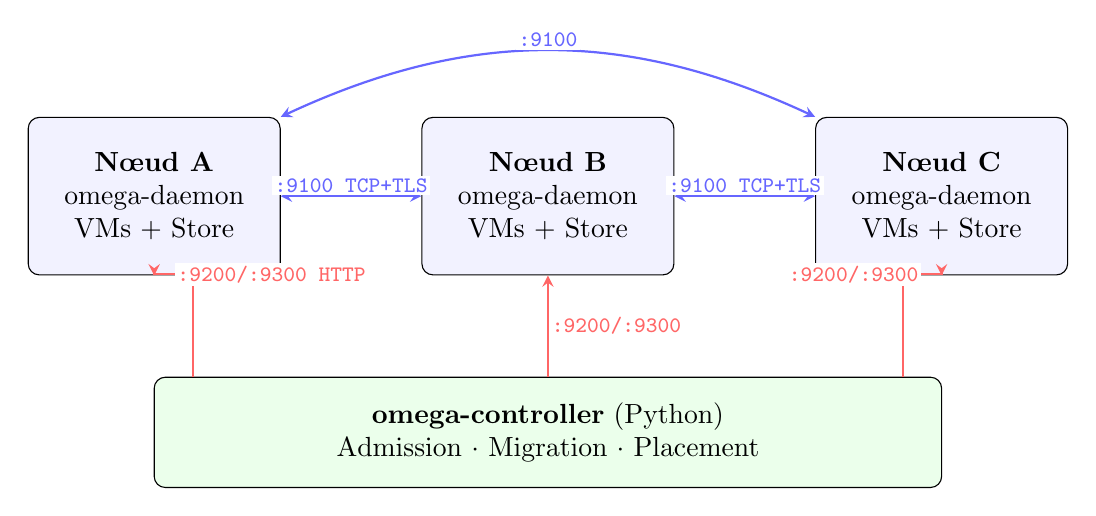
\begin{tikzpicture}[
        node_box/.style={draw, rounded corners, minimum width=3.2cm, minimum height=2cm, align=center, fill=blue!5},
        controller_box/.style={draw, rounded corners, minimum width=10cm, minimum height=1.4cm, align=center, fill=green!8},
        port_label/.style={font=\footnotesize\ttfamily, fill=white, inner sep=1pt},
        >=stealth
    ]
        % Nodes
        \node[node_box] (A) at (0, 0) {\textbf{N\oe{}ud A}\\omega-daemon\\VMs + Store};
        \node[node_box] (B) at (5, 0) {\textbf{N\oe{}ud B}\\omega-daemon\\VMs + Store};
        \node[node_box] (C) at (10, 0) {\textbf{N\oe{}ud C}\\omega-daemon\\VMs + Store};

        % TCP links (peer-to-peer)
        \draw[<->, thick, blue!60] (A.east) -- (B.west) node[port_label, midway, above] {:9100 TCP+TLS};
        \draw[<->, thick, blue!60] (B.east) -- (C.west) node[port_label, midway, above] {:9100 TCP+TLS};
        \draw[<->, thick, blue!60] (A.north east) to[bend left=25] node[port_label, midway, above] {:9100} (C.north west);

        % Controller
        \node[controller_box] (ctrl) at (5, -3) {\textbf{omega-controller} (Python)\\Admission $\cdot$ Migration $\cdot$ Placement};

        % HTTP links (controller to nodes)
        \draw[->, thick, red!60] (ctrl.north west) ++(0.5,0) -- ++(0, 1.3) -| (A.south) node[port_label, near start, right] {:9200/:9300 HTTP};
        \draw[->, thick, red!60] (ctrl.north) -- (B.south) node[port_label, midway, right] {:9200/:9300};
        \draw[->, thick, red!60] (ctrl.north east) ++(-0.5,0) -- ++(0, 1.3) -| (C.south) node[port_label, near start, left] {:9200/:9300};
    \end{tikzpicture}
    \caption{Topologie du cluster omega-remote-paging : paging peer-to-peer (TCP+TLS port~9100) et contr\^ole centralise (HTTP ports~9200/9300).}
    \label{fig:architecture-cluster}
\end{figure}

Trois ports reseau distinct structurent les communications, comme le resume le tableau~\ref{tab:ports-reseau}.

\begin{table}[htbp]
    \centering
    \caption{Ports reseau du systeme et leurs r\^oles.}
    \label{tab:ports-reseau}
    \begin{tabular}{c c p{0.55\linewidth}}
        \toprule
        \textbf{Port} & \textbf{Protocole} & \textbf{R\^ole} \\
        \midrule
        9100 & TCP + TLS & Store inter-n\oe{}uds : protocole binaire (header 20~octets + payload 4~Kio) \\
        9200 & HTTP JSON & API cluster : etat du n\oe{}ud expose au contr\^oleur \\
        9300 & HTTP JSON & Canal de contr\^ole local : quotas, hotplug vCPU, metriques Prometheus \\
        \bottomrule
    \end{tabular}
\end{table}

% -----------------------------------------------------------------------------
\subsection{Composition interne du daemon (\texttt{Arc<NodeState>})}
\label{subsec:composition-daemon}
% -----------------------------------------------------------------------------

Le daemon unifie \texttt{omega-daemon} lance huit t\^aches Tokio au demarrage (fichier \texttt{omega-daemon/src/main.rs}, lignes 57--448). Toutes ces t\^aches partagent un etat central de type \texttt{Arc<NodeState>} (fichier \texttt{omega-daemon/src/node\_state.rs}, ligne~94), qui contient les sous-systemes suivants sans verrou global :

\begin{itemize}
    \item \texttt{store: Arc<PageStore>} --- index \texttt{DashMap} shard\'e pour le stockage des pages distantes.
    \item \texttt{quota\_registry: Arc<QuotaRegistry>} --- quotas RAM par VM, protege par \texttt{RwLock} (lectures non bloquantes entre elles).
    \item \texttt{vcpu\_scheduler: Arc<VcpuScheduler>} --- allocation elastique des vCPU.
    \item \texttt{disk\_io\_scheduler: Arc<DiskIoScheduler>} --- repartition des priorites I/O.
    \item \texttt{gpu\_runtime: Option<Arc<GpuRuntime>>} --- multiplexeur GPU (optionnel).
    \item \texttt{vm\_tracker: Arc<VmTracker>} --- detection des VMs QEMU locales.
\end{itemize}

La communication entre t\^aches utilise trois mecanismes distincts, choisis en fonction du pattern d'acces :

\begin{table}[htbp]
    \centering
    \caption{Mecanismes de synchronisation interne du daemon.}
    \label{tab:sync-mecanismes}
    \begin{tabular}{p{0.22\linewidth} p{0.25\linewidth} p{0.38\linewidth}}
        \toprule
        \textbf{Mecanisme} & \textbf{Utilise par} & \textbf{Justification} \\
        \midrule
        \texttt{DashMap} (sharded) & \texttt{PageStore} & Lectures/ecritures concurrentes de pages sans verrou global \\
        \texttt{RwLock} & \texttt{QuotaRegistry}, \texttt{VcpuScheduler} & Lectures tres frequentes, ecritures rares \\
        \texttt{tokio::mpsc} & \texttt{FaultBus} & Communication unidirectionnelle producteur/consommateur (handler uffd $\to$ eviction engine) \\
        \bottomrule
    \end{tabular}
\end{table}

La section suivante decrit en detail le mecanisme de paging distant qui constitue le c\oe{}ur fonctionnel du systeme.

% =============================================================================
\section{Mécanisme de paging distant}
\label{sec:paging-distant}
% =============================================================================

Le paging distant constitue la primitive technique fondatrice d'\textit{omega-remote-paging} et la contribution la plus directement comparable à l'état de l'art. Le défi conceptuel est double : (i)~intercepter les défauts de page d'une VM sans modifier ni QEMU ni le système invité (objectif~G2), et (ii)~garantir une latence de rappel bornée par 2~ms sur un lien Ethernet commodity (objectif~G1). INFINISWAP~\cite{gu_2017_infiniswap} et Carbink~\cite{zhou_2022_carbink} résolvent ce problème en exposant la mémoire distante comme un périphérique bloc Linux accédé par RDMA~; ces approches atteignent des latences inférieures à 50~\textmu{}s mais exigent un investissement matériel hors de portée d'un cluster Proxmox~VE typique. Cette section présente une alternative entièrement logicielle : interception en espace utilisateur via \texttt{userfaultfd}~\cite{userfaultfd_man}, éviction par approximation CLOCK~\cite{tanenbaum_os,jiang_2005_clockpro}, et transport binaire chiffré sur TCP. Nous montrons que le chemin critique tient dans le budget de latence, et caractérisons les propriétés de la boucle d'éviction adaptative qui prévient le \textit{thrashing}.

% -----------------------------------------------------------------------------
\subsection{Fondement technique : userfaultfd}
\label{subsec:userfaultfd}
% -----------------------------------------------------------------------------

L'interface \texttt{userfaultfd} (User Fault File Descriptor) est un mecanisme du noyau Linux introduit a partir de la version 4.3 qui permet a un programme en espace utilisateur d'intercepter et de resoudre les defauts de page~\cite{userfaultfd_man}. Contrairement au swap Linux classique, qui implique un fichier ou une partition sur disque et un code noyau non modifiable, \texttt{userfaultfd} offre un contr\^ole total depuis l'espace utilisateur.

Le choix de \texttt{userfaultfd} plut\^ot que le swap Linux repose sur trois arguments :

\begin{enumerate}
    \item \textbf{Pas de disque.} Les pages froides sont envoyees vers la RAM d'un autre n\oe{}ud, pas sur un support de stockage persistant. Le swap Linux necessite obligatoirement un fichier ou une partition.
    \item \textbf{Pas de modification du noyau.} L'interface \texttt{userfaultfd} est exposee via \texttt{ioctl()} standard (\texttt{UFFD\_API}, \texttt{UFFDIO\_REGISTER}, \texttt{UFFDIO\_COPY}). Aucun module noyau supplementaire n'est necessaire.
    \item \textbf{Selectivite par VM.} Chaque VM possede son propre file descriptor \texttt{userfaultfd}, ce qui permet de traiter chaque VM independamment et de n'activer le paging distant que sur les VMs qui le necessitent.
\end{enumerate}

L'integration avec QEMU s'effectue via le launcher \texttt{omega-qemu-launcher}, qui injecte un backend memoire de type \texttt{memory-backend-file} base sur un \texttt{memfd} :

\begin{verbatim}
Proxmox -> /usr/bin/kvm -> kvm-omega -> omega-qemu-launcher exec-proxmox
        -> node-a-agent memfd -> QEMU reel + omega-uffd-bridge.so
\end{verbatim}

Le bridge \texttt{omega-uffd-bridge.so} est charge par \texttt{LD\_PRELOAD} dans le processus QEMU reel. Il detecte le mapping \texttt{memfd:omega-vm-<vmid>}, cree le \texttt{userfaultfd}, puis transmet le file descriptor a l'agent via le socket \texttt{/var/lib/omega-qemu/vm-<vmid>/uffd.sock}.

Le flux complet de resolution d'un defaut de page est illustre ci-dessous :

\begin{verbatim}
1. La VM accede a une adresse dont la page est distante
2. Le noyau genere un page fault intercepte par userfaultfd
3. omega-daemon recoit l'evenement via FaultBus
4. GET_PAGE TCP (TLS) envoye au noeud qui stocke la page
5. UFFDIO_COPY : la page (4 096 octets) est copiee en RAM locale
6. La VM reprend son execution --- latence typique < 2 ms sur GbE
\end{verbatim}

La figure~\ref{fig:sequence-pagefault} detaille cette sequence en faisant apparaitre les interactions entre chacun des quatre acteurs impliques.

\begin{figure}[htbp]
    \centering
    \begin{tikzpicture}[
        actorbox/.style={draw, rounded corners=2pt, fill=blue!10,
            minimum width=2.4cm, minimum height=0.65cm,
            align=center, font=\small\bfseries},
        lifeline/.style={dashed, gray!40},
        fwd/.style={-{Stealth[length=3mm]}, thick, blue!70},
        bwd/.style={-{Stealth[length=3mm]}, thick, orange!70},
        sideloop/.style={-{Stealth[length=2.5mm]}, dashed, red!50},
        lbl/.style={font=\scriptsize, fill=white, inner sep=1pt},
    ]
    % ── Actors ────────────────────────────────────────────────────────
    \node[actorbox] (vm)    at (0,   0) {VM\\(QEMU)};
    \node[actorbox] (uffd)  at (3.5, 0) {Noyau\\(\texttt{uffd})};
    \node[actorbox] (dmn)   at (7,   0) {omega-daemon};
    \node[actorbox] (store) at (11,  0) {Store B\\(:9100~TLS)};
    % ── Lifelines ─────────────────────────────────────────────────────
    \draw[lifeline] (0,-0.35)  -- (0,-7.6);
    \draw[lifeline] (3.5,-0.35)-- (3.5,-7.6);
    \draw[lifeline] (7,-0.35)  -- (7,-7.6);
    \draw[lifeline] (11,-0.35) -- (11,-7.6);
    % ── Messages ──────────────────────────────────────────────────────
    \draw[fwd] (0,-1.0) -- (3.5,-1.0)
        node[lbl,midway,above] {\textcircled{1}~page fault (adresse distante)};
    \draw[fwd] (3.5,-1.9) -- (7,-1.9)
        node[lbl,midway,above] {\textcircled{2}~\texttt{UFFD\_EVENT\_PAGEFAULT}};
    \draw[fwd] (7,-3.0) -- (11,-3.0)
        node[lbl,midway,above] {\textcircled{3}~\texttt{GET\_PAGE} (TLS)};
    \draw[bwd] (11,-4.0) -- (7,-4.0)
        node[lbl,midway,above] {\textcircled{4}~\texttt{OK}~+~4\,096~octets};
    \draw[fwd] (7,-5.0) -- (3.5,-5.0)
        node[lbl,midway,above] {\textcircled{5}~\texttt{UFFDIO\_COPY}};
    \draw[bwd] (3.5,-6.0) -- (0,-6.0)
        node[lbl,midway,above] {\textcircled{6}~reprise VM ($<$2\,ms GbE)};
    % ── FaultBus asynchronous notification ────────────────────────────
    \draw[sideloop] (7,-4.4) to[bend left=50]
        node[right, font=\scriptsize, red!60, align=left, xshift=1mm]
            {\texttt{FaultBus}\\[-1pt]\texttt{PageServed}}
        (7,-2.3);
    % ── Time axis ─────────────────────────────────────────────────────
    \draw[-{Stealth}, gray!50] (-1.0,-0.4) -- (-1.0,-6.8)
        node[midway, rotate=90, gray!50, font=\scriptsize, above=2mm] {Temps};
    \end{tikzpicture}
    \caption{Diagramme de sequence : resolution d'un defaut de page distant. La notification \texttt{FaultBus} (en rouge, asynchrone) est envoyee par le daemon a l'etape~\protect\textcircled{4} pour ajuster l'\texttt{AdaptiveInterval} d'eviction.}
    \label{fig:sequence-pagefault}
\end{figure}

% -----------------------------------------------------------------------------
\subsection{Algorithme d'eviction CLOCK}
\label{subsec:eviction-clock}
% -----------------------------------------------------------------------------

Lorsque la pression memoire du n\oe{}ud depasse un seuil configurable, le moteur d'eviction selectionne les pages les moins recemment utilisees pour les envoyer a un store distant. L'algorithme retenu est CLOCK (aussi appele \textit{second chance}), une approximation de LRU (Least Recently Used) a faible co\^ut, largement utilise dans les noyaux de systemes d'exploitation~\cite{tanenbaum_os}.

Le moteur d'eviction est implemente dans le fichier \texttt{omega-daemon/src/eviction\_engine.rs}. Son cycle de fonctionnement est le suivant :

\begin{enumerate}
    \item \textbf{Detection de la pression.} La fonction \texttt{read\_meminfo()} (fichier \texttt{node\_state.rs}, ligne~287) lit \texttt{/proc/meminfo} et extrait \texttt{MemTotal} et \texttt{MemAvailable}. Si l'usage depasse le seuil \texttt{evict\_threshold\_pct} (defaut : 75\,\%, fichier \texttt{config.rs}, ligne~72), l'eviction est declenchee.
    \item \textbf{Identification des VMs candidates.} Le \texttt{VmTracker} fournit la liste des VMs en etat \texttt{Running} sur le n\oe{}ud local (fichier \texttt{eviction\_engine.rs}, lignes~152--156).
    \item \textbf{Selection des pages froides.} Pour chaque VM, les pages sont parcourues circulairement. Chaque page possede un bit de reference : s'il est a 1, il est remis a 0 (seconde chance) ; s'il est a 0, la page est selectionnee pour l'eviction.
    \item \textbf{Envoi au store distant.} La page est envoyee via \texttt{PUT\_PAGE} TCP au n\oe{}ud le moins charge, choisi par \texttt{hash(vm\_id, page\_id) \% num\_stores}.
    \item \textbf{Liberation locale.} L'appel \texttt{madvise(MADV\_DONTNEED)} libere la page du page table local apres envoi.
\end{enumerate}

L'intervalle d'eviction est adaptatif, comme le decrit la section suivante. La figure~\ref{fig:clock-flowchart} presente l'organigramme complet de l'algorithme.

\begin{figure}[htbp]
    \centering
    \begin{tikzpicture}[
        start/.style={draw, ellipse, fill=gray!20, minimum width=2.4cm,
                      minimum height=0.6cm, align=center, font=\small},
        proc/.style={draw, rectangle, rounded corners=2pt, fill=blue!8,
                     minimum width=4.2cm, minimum height=0.62cm,
                     align=center, font=\small},
        dec/.style={draw, diamond, fill=orange!15, minimum width=3cm,
                    minimum height=0.6cm, align=center, font=\small, aspect=2.6},
        arr/.style={-{Stealth[length=2.8mm]}, thick},
        lbl/.style={font=\footnotesize, fill=white, inner sep=1pt},
        node distance=5.5mm,
    ]
    \node[start]  (S)  {Debut cycle};
    \node[proc]   (P1) [below=of S]  {Lire \texttt{/proc/meminfo}};
    \node[dec]    (D1) [below=of P1] {Usage RAM\\$>$ seuil~?};
    \node[proc]   (P2) [below=of D1] {Selectionner VM suivante};
    \node[proc]   (P3) [below=of P2] {Avancer aiguille CLOCK};
    \node[dec]    (D2) [below=of P3] {Bit reference\\$= 1$~?};
    \node[proc]   (Pb) [right=3cm of D2] {Remettre bit ref. a 0\\(seconde chance)};
    \node[proc]   (P5) [below=of D2] {Selectionner page (bit $= 0$)};
    \node[proc]   (P6) [below=of P5] {\texttt{PUT\_PAGE} TCP+TLS\\($\mathrm{hash}(v,p) \bmod N$)};
    \node[proc]   (P7) [below=of P6] {\texttt{madvise(MADV\_DONTNEED)}};
    \node[dec]    (D3) [below=of P7] {Quota atteint\\ou pression OK~?};
    \node[proc]   (P8) [below=of D3] {Attendre \texttt{AdaptiveInterval}};
    \node[start]  (E)  [right=3cm of D3] {Migration\\proposee};
    % Arrows
    \draw[arr] (S) -- (P1);
    \draw[arr] (P1) -- (D1);
    \draw[arr] (D1) -- node[lbl,right] {oui} (P2);
    \draw[arr] (D1.east) -- ++(2.5,0) |- node[lbl,near start,above] {non} (P8);
    \draw[arr] (P2) -- (P3);
    \draw[arr] (P3) -- (D2);
    \draw[arr] (D2) -- node[lbl,right] {non} (P5);
    \draw[arr] (D2) -- node[lbl,above] {oui} (Pb);
    \draw[arr] (Pb.south) -- ++(0,-0.3) -| (P3.east);
    \draw[arr] (P5) -- (P6);
    \draw[arr] (P6) -- (P7);
    \draw[arr] (P7) -- (D3);
    \draw[arr] (D3.east) -- node[lbl,above] {oui} (E);
    \draw[arr] (D3) -- node[lbl,right] {non} (P8);
    \draw[arr] (P8.west) -- ++(-2,0) |- (S.west);
    \end{tikzpicture}
    \caption{Organigramme de l'algorithme CLOCK d'eviction (fichier \texttt{eviction\_engine.rs}). La boucle seconde-chance evite d'evincer les pages recemment accedees.}
    \label{fig:clock-flowchart}
\end{figure}

% -----------------------------------------------------------------------------
\subsection{Le FaultBus : couplage adaptatif eviction/recuperation}
\label{subsec:faultbus}
% -----------------------------------------------------------------------------

Le \texttt{FaultBus} (fichier \texttt{omega-daemon/src/fault\_bus.rs}) est un canal IPC interne qui couple le handler \texttt{userfaultfd} au moteur d'eviction. Sans ce couplage, le moteur d'eviction ne sait pas qu'une page recemment evincee est en train d'etre rappellee, ce qui peut creer un phenomene de ping-pong.

Le bus est implemente comme un canal \texttt{tokio::mpsc} d'une capacite de 4\,096~evenements (fichier \texttt{main.rs}, ligne~297). Trois types d'evenements sont emis (fichier \texttt{fault\_bus.rs}, lignes~38--50) :

\begin{itemize}
    \item \texttt{PageServed\{vm\_id, page\_id, latency\_us\}} : page recuperee depuis le store distant.
    \item \texttt{PageMissing\{vm\_id, page\_id\}} : page absente du store (incoherence).
    \item \texttt{PageLocal\{vm\_id, page\_id\}} : page resolue localement (RAM disponible).
\end{itemize}

Le consommateur \texttt{FaultBusConsumer} (ligne~138) accumule les statistiques sur une fen\^etre glissante temporelle et calcule le debit de fautes distantes (\texttt{remote\_rps}). L'\texttt{AdaptiveInterval} (ligne~243) exploite cette metrique pour ajuster le rythme d'eviction :

\begin{itemize}
    \item \textbf{Mode normal} : intervalle de 10 secondes entre chaque cycle d'eviction.
    \item \textbf{Mode accelere} : intervalle reduit a 2 secondes lorsque \texttt{remote\_rps} depasse le seuil de 5.0 fautes/seconde (fichier \texttt{main.rs}, lignes~305--307).
\end{itemize}

Si le taux de recuperation reste eleve malgre le ralentissement de l'eviction, le daemon genere des recommandations de migration via la \texttt{MigrationPolicy} locale, signalant au contr\^oleur Python que la VM devrait etre deplacee vers un n\oe{}ud moins charge.

% -----------------------------------------------------------------------------
\subsection{Le protocole TCP binaire inter-n\oe{}uds}
\label{subsec:protocole-tcp}
% -----------------------------------------------------------------------------

Les echanges de pages entre n\oe{}uds utilisent un protocole binaire proprietaire sur TCP, concu pour minimiser la latence de parsing. Chaque trame comporte un en-tete fixe de 20~octets suivi d'un payload variable. Le format est defini dans le fichier \texttt{docs/protocol.md} et implemente dans \texttt{node-bc-store/src/protocol.rs} :

\begin{verbatim}
 0                   1                   2                   3
 0 1 2 3 4 5 6 7 8 9 0 1 2 3 4 5 6 7 8 9 0 1 2 3 4 5 6 7 8 9 0 1
+-+-+-+-+-+-+-+-+-+-+-+-+-+-+-+-+-+-+-+-+-+-+-+-+-+-+-+-+-+-+-+-+
|      magic (0x524D = "RM")    |   opcode      |     flags     |
+-+-+-+-+-+-+-+-+-+-+-+-+-+-+-+-+-+-+-+-+-+-+-+-+-+-+-+-+-+-+-+-+
|                           vm_id (u32)                         |
+-+-+-+-+-+-+-+-+-+-+-+-+-+-+-+-+-+-+-+-+-+-+-+-+-+-+-+-+-+-+-+-+
|                                                               |
|                          page_id (u64)                        |
+-+-+-+-+-+-+-+-+-+-+-+-+-+-+-+-+-+-+-+-+-+-+-+-+-+-+-+-+-+-+-+-+
|                       payload_len (u32)                       |
+-+-+-+-+-+-+-+-+-+-+-+-+-+-+-+-+-+-+-+-+-+-+-+-+-+-+-+-+-+-+-+-+
|               payload (0 a 8 192 octets)                      |
+-+-+-+-+-+-+-+-+-+-+-+-+-+-+-+-+-+-+-+-+-+-+-+-+-+-+-+-+-+-+-+-+
\end{verbatim}

Tous les champs multi-octets sont en big-endian. Le champ \texttt{magic} (\texttt{0x524D} pour \og RM \fg{} --- \textit{Remote Memory}) identifie le protocole. Le champ \texttt{flags} reserve le bit~0 pour la compression LZ4~\cite{lz4_compression} (non activee par defaut).

Les opcodes sont structures en deux categories :

\begin{table}[htbp]
    \centering
    \caption{Opcodes du protocole TCP de paging.}
    \label{tab:opcodes-tcp}
    \begin{tabular}{c c c p{0.40\linewidth}}
        \toprule
        \textbf{Opcode} & \textbf{Valeur} & \textbf{Sens} & \textbf{Description} \\
        \midrule
        \texttt{PING} & \texttt{0x01} & $\to$ & Verification de connectivite \\
        \texttt{PUT\_PAGE} & \texttt{0x10} & $\to$ & Stocke une page (payload = 4\,096~octets) \\
        \texttt{GET\_PAGE} & \texttt{0x11} & $\to$ & Recupere une page \\
        \texttt{DELETE\_PAGE} & \texttt{0x12} & $\to$ & Supprime une page \\
        \texttt{STATS\_REQUEST} & \texttt{0x20} & $\to$ & Demande les statistiques du store \\
        \midrule
        \texttt{PONG} & \texttt{0x02} & $\leftarrow$ & Reponse a \texttt{PING} \\
        \texttt{OK} & \texttt{0x80} & $\leftarrow$ & Operation reussie (+ donnees si \texttt{GET}) \\
        \texttt{NOT\_FOUND} & \texttt{0x81} & $\leftarrow$ & Page absente du store \\
        \texttt{ERROR} & \texttt{0x82} & $\leftarrow$ & Erreur (message UTF-8 dans le payload) \\
        \texttt{STATS\_RESPONSE} & \texttt{0x21} & $\leftarrow$ & Statistiques (JSON dans le payload) \\
        \bottomrule
    \end{tabular}
\end{table}

Le choix d'un protocole binaire fixe plut\^ot que JSON ou Protocol Buffers est motive par :

\begin{itemize}
    \item \textbf{Parsing $O(1)$.} L'en-tete est lu en une seule operation de 20~octets, sans analyse lexicale.
    \item \textbf{Protection DoS.} Le payload est limite a $2 \times \texttt{PAGE\_SIZE} = 8\,192$ octets. Un attaquant ne peut pas envoyer de trames geantes.
    \item \textbf{Latence deterministe.} La deserialization d'un JSON variable ajoute une variance de latence incompatible avec la contrainte C1.
\end{itemize}

La distribution des pages entre stores est deterministe : \texttt{hash(vm\_id, page\_id) \% num\_stores}. Ce schema evite toute coordination inter-n\oe{}uds pour localiser une page. Le facteur de replication est configurable (defaut : 2 copies via la variable d'environnement \texttt{OMEGA\_REPLICATION\_FACTOR}).

% -----------------------------------------------------------------------------
\subsection{Securisation du canal : TLS TOFU}
\label{subsec:tls-tofu}
% -----------------------------------------------------------------------------

Les pages memoire des VMs contiennent potentiellement des donnees sensibles (mots de passe, cles, donnees applicatives). Sans chiffrement, tout equipement reseau intermediaire peut lire ou modifier les pages en transit.

Le module TLS (fichier \texttt{omega-daemon/src/tls.rs}) implemente un chiffrement du canal TCP (port~9100) avec les caracteristiques suivantes :

\begin{itemize}
    \item \textbf{Certificat auto-signe} : au premier demarrage, une paire de cles RSA-2048 et un certificat X.509 sont generes automatiquement via la bibliotheque \texttt{rcgen} et sauvegardes dans \texttt{/etc/omega-store/tls/} (\texttt{cert.pem} + \texttt{key.pem}).
    \item \textbf{Modele TOFU} (\textit{Trust On First Use}) : la verification des pairs s'effectue par empreinte SHA-256 du certificat, fixee dans la configuration. Aucune autorite de certification n'est necessaire, ce qui simplifie le deploiement.
    \item \textbf{TLS~1.3} : le chiffrement utilise AES-256-GCM via la bibliotheque \texttt{rustls}~\cite{rustls_crate} (avec le backend \texttt{ring}).
\end{itemize}

Le surcout de performance a ete mesure et documente (fichier \texttt{tls.rs}, lignes 30--35) :

\begin{itemize}
    \item Handshake TLS~1.3 : $\sim$0,5~ms (une seule fois par connexion).
    \item Chiffrement AES-256-GCM : $\sim$0,3~ns/octet $= \sim$1,2~\textmu{}s/page (4~Kio).
    \item Surcout total par page : $< 2$~\textmu{}s, a comparer a la latence reseau de 50--500~\textmu{}s.
\end{itemize}

L'impact est donc negligeable sur les performances en pratique, ce qui justifie l'activation systematique du chiffrement.

% -----------------------------------------------------------------------------
\subsection{Thin-provisioning par balloon virtio}
\label{subsec:balloon}
% -----------------------------------------------------------------------------

Le mecanisme de balloon virtio permet d'ajuster dynamiquement la quantite de RAM physique consommee par une VM sans l'arreter~\cite{qemu_balloon,waldspurger_2002}. Le module \texttt{balloon.rs} (fichier \texttt{omega-daemon/src/balloon.rs}) implemente deux composants complementaires :

\begin{enumerate}
    \item \textbf{\texttt{BalloonMonitor}} : lit les statistiques internes de chaque VM via le protocole QMP (socket Unix \texttt{/var/run/qemu-server/\{vmid\}.qmp}) toutes les 15~secondes (fichier \texttt{main.rs}, ligne~353). Les statistiques incluent la RAM libre c\^ote guest (\texttt{free\_pct}), la RAM totale, et le nombre de defauts de page majeurs. Si \texttt{free\_pct} descend sous 20\,\% (fichier \texttt{main.rs}, ligne~357), un avertissement est emis.

    \item \textbf{\texttt{BalloonManager}} : gonfle proactivement le balloon des guests sur-provisionnes pour recuperer la RAM inutilisee, et le degonfle lorsqu'un guest est sous pression. La reconciliation s'effectue toutes les 30~secondes (fichier \texttt{main.rs}, ligne~392).
\end{enumerate}

Le lien avec le systeme de quotas est direct : lorsque le balloon reduit la RAM physique du guest a \texttt{balloon\_actual\_mib}, le budget distant peut cro\^itre dynamiquement :

\begin{equation}
    \label{eq:balloon-quota}
    \texttt{remote\_budget} = \texttt{max\_mem} - \texttt{balloon\_actual}
\end{equation}

Cette mise a jour est realisee par l'appel \texttt{apply\_balloon\_update(vmid, actual\_mib)} qui declenche \texttt{adjust\_for\_balloon()} dans le \texttt{QuotaRegistry} (fichier \texttt{quota.rs}, lignes~123--143).

% =============================================================================
\section{Contrôle d'admission et système de quotas}
\label{sec:quotas}
% =============================================================================

L'admission et le quota constituent la frontière formelle de l'isolation entre VMs. Cette section répond à deux questions complémentaires : (1)~comment décider, à l'arrivée d'une nouvelle VM, sur quel nœud elle peut être placée et avec quel partage local/distant~? (2)~comment garantir, en régime d'exploitation, qu'une VM ne dépasse jamais son budget négocié, quelles que soient les rafales de défauts de page subies~? La réponse à la seconde question prend la forme d'une proposition formelle (\autoref{prop:quota-invariant}) qui pose le fondement de la sûreté du système et justifie la contrainte~G5 énoncée à la section~\ref{subsec:contraintes-nf}.

% -----------------------------------------------------------------------------
\subsection{Formalisation et démonstration de l'invariant de quota}
\label{subsec:invariant-quota}
% -----------------------------------------------------------------------------

Le système de quotas constitue le fondement formel de la sûreté du système. Nous commençons par définir précisément la notion de quota, puis énonçons et démontrons l'invariant central.

\begin{definition}[Quota d'une VM]
\label{def:quota}
Pour toute VM $v \in \mathcal{V}_t$, on définit son \emph{quota} $Q(v)$ comme le quadruplet
\[
    Q(v) \;=\; \bigl(\, M_{\max}(v),\; M_{\ell}(v),\; M_r(v),\; U_r^t(v) \,\bigr),
\]
où $M_{\max}(v)$ est le budget mémoire total négocié à l'admission, $M_{\ell}(v) \leq M_{\max}(v)$ le budget alloué sur $\mathrm{host}(v)$, $M_r(v) = M_{\max}(v) - M_{\ell}(v)$ le budget distant maximal, et $U_r^t(v) \leq M_r(v)$ la consommation distante effective à l'instant $t$. Toutes les grandeurs sont exprimées en mébi-octets.
\end{definition}

L'égalité $M_r(v) = M_{\max}(v) - M_{\ell}(v)$ est imposée par construction à l'admission. Cette répartition exhaustive du quota entre local et distant exclut tout sur-engagement.

\begin{proposition}[Invariant de quota multi-ressources]
\label{prop:quota-invariant}
À tout instant $t$ et pour toute VM $v \in \mathcal{V}_t$~:
\begin{equation}
    \label{eq:quota-invariant}
    L_t(v) \;+\; U_r^t(v) \;\leq\; M_{\max}(v).
\end{equation}
\end{proposition}

\begin{proof}[Esquisse]
La démonstration repose sur deux contrôles redondants couvrant chacun un point d'entrée distinct vers la consommation de quota.

\textbf{(i) Admission.} Lorsqu'une VM $v$ est créée, le contrôleur d'admission (section~\ref{subsec:admission-ram}) choisit un nœud cible $n = \mathrm{host}(v)$ tel que $M_{\ell}(v) \leq R_{\text{libre}}(n)$. Le système d'exploitation hôte garantit alors $L_t(v) \leq M_{\ell}(v)$ pour tout $t$, par mise en application de la limite cgroup~v2 \texttt{memory.max}~\cite{cgroups_v2_doc}.

\textbf{(ii) Écriture de page distante.} À chaque opération \texttt{PUT\_PAGE} (section~\ref{subsec:protocole-tcp}), le \texttt{QuotaRegistry} vérifie la condition
\begin{equation}
    \label{eq:check-put}
    U_r^t(v) + \left\lceil \frac{p}{2^{20}} \right\rceil \;\leq\; M_r(v),
\end{equation}
où $p$ est la taille de la page (4~096~octets). Toute violation entraîne le rejet \texttt{QuotaCheck::Exceeded} et l'écriture n'a pas lieu. Il en découle $U_r^t(v) \leq M_r(v)$ à tout instant.

En combinant (i) et (ii) avec la définition $M_r(v) = M_{\max}(v) - M_{\ell}(v)$ de la \autoref{def:quota}, on obtient~:
\[
    L_t(v) + U_r^t(v) \;\leq\; M_{\ell}(v) + M_r(v) \;=\; M_{\max}(v),
\]
ce qui établit l'inéquation~(\ref{eq:quota-invariant}). \qedhere
\end{proof}

\paragraph{Conséquence opérationnelle.}
La \autoref{prop:quota-invariant} garantit qu'aucune VM ne peut, par accumulation de pages distantes, dépasser son budget mémoire négocié, indépendamment du nombre de défauts de page subis ou du choix du nœud store. Cette propriété est cruciale pour la facturation et l'isolation des locataires dans un cluster multi-tenants.

\paragraph{Implémentation.}
Le \texttt{QuotaRegistry} (fichier \texttt{omega-daemon/src/quota.rs}) maintient une table \texttt{HashMap} associant chaque \texttt{vm\_id} à sa structure \texttt{VmQuota}, protégée par un \texttt{RwLock}. Le choix d'un verrou en lecture/écriture privilégie les lectures fréquentes (chaque \texttt{PUT\_PAGE} appelle \texttt{check\_put()}) en les rendant non bloquantes entre elles, tout en sérialisant les écritures rares (configuration initiale, ajustement balloon, suppression après migration).

% -----------------------------------------------------------------------------
\subsection{Flux de configuration d'un quota}
\label{subsec:flux-quota}
% -----------------------------------------------------------------------------

La configuration d'un quota suit un flux en quatre etapes :

\begin{verbatim}
1. Controller calcule : local_budget = RAM disponible sur le noeud cible
                        remote_budget = max_mem - local_budget
2. POST /control/vm/{vmid}/quota -> QuotaRegistry.set()
3. Hook Proxmox (post-start) declenche la configuration initiale
4. Ajustements dynamiques : balloon, migration, arret VM
\end{verbatim}

Apres une migration, \texttt{record\_delete\_vm()} (ligne~259) remet a zero la consommation distante. Apres l'arr\^et d'une VM, \texttt{remove()} (ligne~202) supprime completement le quota.

% -----------------------------------------------------------------------------
\subsection{Admission RAM a l'echelle du cluster}
\label{subsec:admission-ram}
% -----------------------------------------------------------------------------

L'\texttt{AdmissionController} (fichier \texttt{controller/controller/admission.py}) coordonne l'admission des nouvelles VMs a l'echelle du cluster. Pour chaque demande de creation de VM, il effectue les verifications suivantes :

\begin{enumerate}
    \item \textbf{Capacite totale.} La somme des RAM disponibles sur tous les n\oe{}uds du cluster doit etre superieure ou egale a \texttt{vm.max\_mem}.
    \item \textbf{Selection du n\oe{}ud cible.} Le moteur de placement topologique (fichier \texttt{topology\_placement.py}) calcule un score multi-criteres pour chaque n\oe{}ud candidat :
    \begin{equation}
        \label{eq:placement-score}
        \text{score}(n) = 0{,}50 \times r_{\text{RAM}} + 0{,}25 \times r_{\text{topo}} + 0{,}15 \times r_{\text{CPU}} + 0{,}10 \times r_{\text{migr}}
    \end{equation}
    o\`u $r_{\text{RAM}}$ est la RAM libre normalisee, $r_{\text{topo}}$ le score topologique (1,0 si meme rack, 0,7 si meme zone, 0,3 si inter-zone), $r_{\text{CPU}} = 1 - \text{cpu\_usage}$, et $r_{\text{migr}} = 1 / (1 + \text{migrations\_en\_cours})$.
    \item \textbf{Veto.} Si aucun n\oe{}ud ne peut accueillir la VM sans depasser 80\,\% de RAM utilisee, l'admission est refusee.
\end{enumerate}

% -----------------------------------------------------------------------------
\subsection{Admission vCPU et GPU}
\label{subsec:admission-cpu-gpu}
% -----------------------------------------------------------------------------

L'admission des ressources CPU est geree par le \texttt{ClusterVcpuPoolPlanner} (fichier \texttt{controller/controller/cpu\_admission.py}). Il selectionne le n\oe{}ud avec le plus de slots vCPU libres et verifie que l'overcommit ne depasse pas $3\times$ le nombre de c\oe{}urs physiques.

L'admission GPU est geree par le \texttt{GpuAdmissionController} (fichier \texttt{controller/controller/gpu\_admission.py}). Pour chaque VM necessitant un GPU, il verifie que le n\oe{}ud cible dispose de suffisamment de VRAM libre :

\begin{equation}
    \texttt{gpu\_free\_vram\_mib} \geq \texttt{vm.gpu\_budget\_mib}
\end{equation}

Si aucun n\oe{}ud GPU n'a assez de VRAM, l'admission est refusee. Ces trois contr\^oles (RAM, vCPU, GPU) sont evalues conjointement : la VM n'est admise que si les trois sont satisfaits.

% =============================================================================
\section{Ordonnanceur vCPU élastique}
\label{sec:vcpu-scheduler}
% =============================================================================

Le second axe de mutualisation concerne la capacité de calcul. Les ordonnanceurs commerciaux tels que VMware~DRS~\cite{gulati_2012_drs} traitent l'allocation vCPU comme une décision statique prise à la création de la VM~; toute adaptation ultérieure requiert une intervention administrative. Cette section présente un ordonnanceur \emph{élastique} qui ajuste dynamiquement le nombre de vCPU alloués à chaque VM en fonction de sa charge réelle, observée à 1~ms de granularité, par lecture des compteurs cgroup~v2~\cite{cgroups_v2_doc}. La stratégie privilégie le rééquilibrage local (hot-plug ou pondération \texttt{cpu.weight}) avant d'escalader vers une migration cluster-wide~; ce principe d'escalade progressive limite le coût des décisions et préserve la stabilité du système (cf. la cascade illustrée en figure~\ref{fig:migration-cascade}).

% -----------------------------------------------------------------------------
\subsection{Modele d'allocation elastique}
\label{subsec:modele-vcpu}
% -----------------------------------------------------------------------------

Le modele est defini dans le fichier \texttt{omega-daemon/src/vcpu\_scheduler.rs} par les constantes suivantes (lignes 46--70) :

\begin{itemize}
    \item \texttt{VCPU\_PER\_PCPU = 3} : chaque c\oe{}ur physique expose 3 slots virtuels.
    \item \texttt{MAX\_VMS\_PER\_SLOT = 3} : un slot vCPU peut etre partage entre au maximum 3 VMs simultanement (le scheduler CFS du noyau Linux gere le decoupage temporel).
    \item \texttt{HOTPLUG\_TRIGGER\_PCT = 80.0} : seuil d'utilisation CPU declenchant un hotplug.
    \item \texttt{DOWNSCALE\_TRIGGER\_PCT = 35.0} : seuil sous lequel un retrait progressif est envisage.
    \item \texttt{DOWNSCALE\_STABLE\_SECS = 60} : duree minimale de faible charge avant retrait.
    \item \texttt{STEAL\_THRESHOLD\_PCT = 10.0} : seuil de steal time declenchant une migration prioritaire.
\end{itemize}

Chaque VM est modelisee par la structure \texttt{VmVcpuState} (ligne~92), qui maintient :

\begin{itemize}
    \item \texttt{min\_vcpus} : nombre de vCPU au demarrage (lu depuis \texttt{vcpus:} dans la configuration Proxmox).
    \item \texttt{max\_vcpus} : plafond demande ($= \texttt{sockets} \times \texttt{cores}$, lu depuis le fichier \texttt{.conf}).
    \item \texttt{current\_vcpus} : vCPU actuellement alloues ($\texttt{min} \leq \texttt{current} \leq \texttt{max}$).
    \item \texttt{cpu\_usage\_pct} : utilisation CPU moyenne sur les 60 dernieres secondes.
    \item \texttt{steal\_pct} : pourcentage de temps CPU vole par l'hyperviseur.
    \item \texttt{cpu\_weight} : poids cgroup \texttt{cpu.weight} actuellement applique.
\end{itemize}

% -----------------------------------------------------------------------------
\subsection{Mecanismes de hotplug et downscale}
\label{subsec:hotplug-downscale}
% -----------------------------------------------------------------------------

Le hotplug de vCPU est declenche lorsque l'une des deux conditions suivantes est detectee :

\begin{enumerate}
    \item \texttt{avg\_cpu\_pct} $\geq$ \texttt{HOTPLUG\_TRIGGER\_PCT} (80\,\%).
    \item \texttt{throttle\_ratio} $\geq$ \texttt{THROTTLE\_THRESHOLD} (10\,\%, fichier \texttt{cgroup\_cpu\_monitor.rs}, ligne~49).
\end{enumerate}

La detection s'effectue a deux frequences :

\begin{itemize}
    \item \textbf{Haute frequence (1~ms)} : le \texttt{CgroupCpuMonitor} (fichier \texttt{cgroup\_cpu\_monitor.rs}) lit \texttt{cpu.stat} de chaque VM toutes les millisecondes via une fen\^etre glissante de 100~echantillons (\texttt{WINDOW\_SIZE = 100}, ligne~45). Il emet un \texttt{CpuPressureEvent} lorsque les seuils sont depasses. Ce monitor est implemente en Rust plut\^ot qu'en Python car le GIL empeche la parallelisation des lectures cgroups sous charge (20+ VMs).
    \item \textbf{Basse frequence (100~ms+)} : la boucle principale de monitoring CPU (fichier \texttt{main.rs}, lignes~170--292) lit \texttt{cpu.stat} et calcule l'usage par difference de compteurs.
\end{itemize}

La realisation du hotplug s'effectue via le protocole QMP (QEMU Machine Protocol) :

\begin{verbatim}
hotplug   : device_add cpu,id=cpu{n}  -> HotplugResult::Added{new_count}
hot-unplug: device_del cpu{n}         -> HotplugResult::Removed{new_count}
\end{verbatim}

Si le hotplug QMP echoue (plus de slots disponibles), le scheduler annule sa reservation interne via \texttt{rollback\_hotplug()} et genere une decision \texttt{VcpuDecision::MigrateRequired} (fichier \texttt{main.rs}, lignes~735--753).

Le downscale suit un processus inverse : lorsque \texttt{avg\_cpu\_pct} $<$ 35\,\% depuis au moins 60~secondes (\texttt{DOWNSCALE\_STABLE\_SECS}), un vCPU est retire via \texttt{device\_del}.

% -----------------------------------------------------------------------------
\subsection{Partage CPU local temporaire}
\label{subsec:partage-cpu}
% -----------------------------------------------------------------------------

Avant de recourir a la migration, le systeme tente de reequilibrer les ressources CPU localement via trois mecanismes successifs (fichier \texttt{main.rs}, fonction \texttt{reconcile\_local\_cpu\_sharing}, lignes~861--950) :

\begin{enumerate}
    \item \textbf{Reclamation locale.} Un donor idle (VM durablement sous-utilisee) libere un vCPU via hot-unplug. Ce vCPU est immediatement attribue au borrower (VM sous pression) via hotplug.
    \item \textbf{Partage via \texttt{cpu.weight}.} Les poids cgroup sont ajustes :
    \begin{itemize}
        \item Borrower (VM sous pression) : \texttt{BOOSTED\_CPU\_WEIGHT = 200} (ligne~66).
        \item Donor (VM idle) : \texttt{DONOR\_CPU\_WEIGHT = 50} (ligne~69).
        \item VM nominale : \texttt{DEFAULT\_CPU\_WEIGHT = 100} (ligne~64).
    \end{itemize}
    Une contrainte de securite empeche un donor de perdre trop de capacite : son steal time doit rester inferieur a \texttt{DONOR\_SAFE\_STEAL\_PCT = 5.0\,\%} (ligne~73).
    \item \textbf{Migration.} Si la saturation persiste malgre le partage local, la VM est signalee comme candidate a la migration.
\end{enumerate}

% -----------------------------------------------------------------------------
\subsection{Escalade vers la migration}
\label{subsec:escalade-migration}
% -----------------------------------------------------------------------------

Le scheduler ne decide jamais d'une migration de maniere autonome. Il expose les signaux de pression via le snapshot \texttt{NodeStatus} (fichier \texttt{node\_state.rs}), que le contr\^oleur Python interroge periodiquement via \texttt{GET /api/status}. Deux conditions declenchent l'escalade :

\begin{enumerate}
    \item \texttt{steal\_pct} $>$ \texttt{STEAL\_THRESHOLD\_PCT} (10\,\%) de maniere persistante.
    \item Aucun slot hotpluggable disponible et la VM est encore throttlee.
\end{enumerate}

Le contr\^oleur Python evalue alors la migration en tenant compte de l'ensemble des ressources du cluster (section~\ref{sec:migration}).

% =============================================================================
\section{Arbitrage des entrées/sorties disque}
\label{sec:disk-scheduler}
% =============================================================================

L'hypothèse~\ref{hyp:reseau-stockage} stipule que le stockage des disques virtuels repose sur Ceph~RBD~\cite{ceph_doc}, ce qui élimine le besoin de migrer les disques entre nœuds. Cette hypothèse ne dispense toutefois pas le système d'arbitrer la contention locale~: les caches I/O, journaux et opérations de \textit{flush} restent traités par le noyau du nœud hôte et créent des goulots d'étranglement lorsque plusieurs VMs sollicitent simultanément le sous-système de stockage. Cette section décrit l'arbitrage \texttt{io.weight} basé sur la pression mesurée par PSI~\cite{psi_doc}, et précise les seuils déclencheurs dérivés de mesures expérimentales.

% -----------------------------------------------------------------------------
\subsection{Lecture de la pression I/O via PSI}
\label{subsec:psi-io}
% -----------------------------------------------------------------------------

La pression I/O du n\oe{}ud est mesuree via PSI (Pressure Stall Information), un mecanisme du noyau Linux 4.20+ qui quantifie le temps passe a attendre des ressources~\cite{psi_doc}. Le fichier \texttt{/proc/pressure/io} expose la metrique \texttt{some.avg10} : le pourcentage du temps (sur 10~secondes) durant lequel au moins un thread attendait de l'I/O.

L'interpretation est la suivante (documentee dans \texttt{docs/metrics.md}, lignes~96--101) :

\begin{table}[htbp]
    \centering
    \caption{Interpretation des niveaux de pression PSI I/O.}
    \label{tab:psi-interpretation}
    \begin{tabular}{c p{0.55\linewidth}}
        \toprule
        \textbf{Valeur \texttt{some.avg10}} & \textbf{Interpretation} \\
        \midrule
        0 -- 1\,\% & Aucune pression \\
        1 -- 5\,\% & Pression moderee \\
        5 -- 10\,\% & Pression elevee (seuil de declenchement) \\
        $>$ 10\,\% & Pression critique \\
        \bottomrule
    \end{tabular}
\end{table}

Le module \texttt{io\_cgroup.rs} (fichier \texttt{omega-daemon/src/io\_cgroup.rs}) lit la pression via \texttt{CgroupIoController::read\_node\_pressure\_pct()}.

% -----------------------------------------------------------------------------
\subsection{Politique de poids \texttt{io.weight}}
\label{subsec:io-weight}
% -----------------------------------------------------------------------------

Le scheduler disque (fichier \texttt{omega-daemon/src/disk\_io\_scheduler.rs}) definit trois niveaux de poids (lignes 17--19) :

\begin{itemize}
    \item \texttt{DEFAULT\_IO\_WEIGHT = 100} : poids nominal de toute VM.
    \item \texttt{BOOSTED\_IO\_WEIGHT = 200} : poids accorde a une VM active sous pression.
    \item \texttt{DONOR\_IO\_WEIGHT = 50} : poids reduit pour une VM durablement idle.
\end{itemize}

Le declenchement du boosting requiert deux conditions simultanees (lignes~67--69 de la structure \texttt{VmDiskState}) :

\begin{enumerate}
    \item La pression I/O du n\oe{}ud depasse \texttt{DISK\_PRESSURE\_TRIGGER\_PCT = 5.0\,\%} (PSI \texttt{some.avg10}).
    \item Le debit total de la VM depasse \texttt{DISK\_BORROWER\_TRIGGER\_BPS = 8~Mio/s}.
\end{enumerate}

Une VM est consideree idle lorsque son debit total est inferieur a \texttt{DISK\_IDLE\_BPS = 512~Kio/s} depuis au moins \texttt{DISK\_IDLE\_STABLE\_SECS = 60~s} (lignes 22--23).

Si \texttt{io.weight} n'est pas disponible dans le cgroup de la VM (backend non supporte), le systeme effectue un fallback gracieux : la methode \texttt{mark\_io\_control\_unsupported()} desactive le contr\^ole pour cette VM et consigne la raison dans les logs (fichier \texttt{main.rs}, lignes~979--1004). La telemetrie et la migration restent actives.

% -----------------------------------------------------------------------------
\subsection{Lecture des compteurs reels \texttt{io.stat}}
\label{subsec:io-stat}
% -----------------------------------------------------------------------------

Le module \texttt{io\_cgroup.rs} lit les compteurs I/O reels depuis le fichier cgroup v2 \texttt{io.stat} de chaque VM. Le format est \texttt{<major>:<minor> rbytes=... wbytes=...}. Le debit en octets/seconde est calcule par difference de snapshots successifs :

\begin{equation}
    \text{read\_bps} = \frac{\texttt{rbytes\_now} - \texttt{rbytes\_before}}{\Delta t_{\mu s}} \times 10^6
\end{equation}

Ces valeurs alimentent le scheduler disque et sont exposees dans le snapshot \texttt{VmStatusEntry} (fichier \texttt{node\_state.rs}, lignes~68--70), rendant les debits I/O par VM visibles au contr\^oleur Python pour les decisions de migration.

% =============================================================================
\section{Multiplexage du GPU}
\label{sec:gpu-multiplexer}
% =============================================================================

Les accélérateurs graphiques constituent une ressource fondamentalement différente de la RAM ou du CPU : leur architecture matérielle interdit le partage transparent entre processus indépendants, et les solutions de virtualisation existantes sont soit propriétaires (vGPU NVIDIA), soit dépendantes du matériel (SR-IOV). Cette section présente un multiplexeur applicatif en espace utilisateur qui contourne ces limitations en sérialisant les commandes GPU au niveau d'un démon arbitre, et en associant à chaque VM un budget VRAM mis en application par contrôle d'admission. L'approche est inspirée des \textit{rendering proxies} utilisés dans les systèmes de \textit{thin clients}, étendue ici à la coordination cluster-wide via le contrôleur Python.

% -----------------------------------------------------------------------------
\subsection{Problematique du partage GPU}
\label{subsec:problematique-gpu}
% -----------------------------------------------------------------------------

Dans un cluster Proxmox standard, un GPU physique ne peut etre assigne qu'a une seule VM via le mecanisme de PCI passthrough. Cette exclusivite est probl\'ematique lorsque plusieurs VMs necessite des capacites GPU (inference IA, rendu graphique) mais qu'aucune n'utilise le GPU a pleine capacite en permanence.

Les alternatives considerees et ecartees sont :

\begin{itemize}
    \item \textbf{SR-IOV (Single Root I/O Virtualization)} : necessite un GPU compatible et un support pilote, limite a certaines gammes NVIDIA/AMD.
    \item \textbf{vGPU (NVIDIA GRID/MIG)} : solution proprietaire necessitant des licences co\^uteuses.
    \item \textbf{Multiplexeur en espace utilisateur} (retenu) : un daemon intermediaire arbitre les acces GPU via un socket Unix, sans modification du pilote noyau.
\end{itemize}

% -----------------------------------------------------------------------------
\subsection{Architecture du multiplexeur}
\label{subsec:architecture-mux}
% -----------------------------------------------------------------------------

Le multiplexeur (fichier \texttt{omega-daemon/src/gpu\_multiplexer.rs}) ecoute sur un socket Unix (\texttt{/run/omega/gpu.sock}) et gere les requetes GPU de toutes les VMs du n\oe{}ud. Son architecture interne repose sur trois composants :

\begin{enumerate}
    \item \textbf{File de priorite.} Les commandes GPU sont ordonnees par un \texttt{BinaryHeap} (ligne~31) selon deux criteres :
    \begin{itemize}
        \item Priorite du message : \texttt{RealTime} (3) $>$ \texttt{High} (2) $>$ \texttt{Normal} (1) $>$ \texttt{Low} (0).
        \item Timestamp d'arrivee (FIFO a meme priorite).
    \end{itemize}

    \item \textbf{Worker unique.} Un thread unique consomme la file et soumet les commandes au GPU physique. Cette serialisation est necessaire car la plupart des pilotes GPU ne sont pas thread-safe (lignes~27--29 du fichier \texttt{gpu\_multiplexer.rs}).

    \item \textbf{Budget VRAM par VM.} Chaque VM dispose d'un \texttt{VmVramBudget} (ligne~47) qui definit un budget total en Mio et suit la VRAM actuellement allouee. La methode \texttt{can\_alloc\_bytes()} (ligne~67) verifie que toute allocation respecte le budget :
    \begin{equation}
        \texttt{used\_mib} + \left\lceil\frac{\texttt{bytes}}{1\,048\,576}\right\rceil \leq \texttt{budget\_mib}
    \end{equation}
\end{enumerate}

% -----------------------------------------------------------------------------
\subsection{Protocole GPU binaire}
\label{subsec:protocole-gpu}
% -----------------------------------------------------------------------------

Le protocole entre les VMs et le multiplexeur utilise un format binaire proprietaire avec un header fixe de 22~octets (fichier \texttt{omega-daemon/src/gpu\_protocol.rs}) :

\begin{verbatim}
+----------+----------+----------+----------+----------+
| magic 4B | vers. 1B | type  1B | vm_id 4B |  seq 4B  |
+----------+----------+----------+----------+----------+
| payload_len 4B | priority 1B | reserved 3B            |
+----------+----------+-----------------------------------+
| payload (variable)                                      |
+---------------------------------------------------------+
\end{verbatim}

Le nombre magique est \texttt{0x4F4D4750} (\og OMGP \fg{} pour \textit{Omega GPU Protocol}, fichier \texttt{gpu\_protocol.rs}, ligne~32). Les types de messages sont definis par l'enumeration \texttt{MsgType} (lignes~39--49) :

\begin{table}[htbp]
    \centering
    \caption{Types de messages du protocole GPU.}
    \label{tab:gpu-msg-types}
    \begin{tabular}{c c c p{0.40\linewidth}}
        \toprule
        \textbf{Type} & \textbf{Valeur} & \textbf{Sens} & \textbf{Description} \\
        \midrule
        \texttt{GPU\_CMD} & \texttt{0x01} & VM$\to$GPU & Commande GPU brute \\
        \texttt{GPU\_RESULT} & \texttt{0x02} & GPU$\to$VM & Resultat d'une commande \\
        \texttt{GPU\_ALLOC} & \texttt{0x03} & VM$\to$GPU & Allocation VRAM \\
        \texttt{GPU\_ALLOC\_RESP} & \texttt{0x04} & GPU$\to$VM & Handle VRAM alloue \\
        \texttt{GPU\_FREE} & \texttt{0x05} & VM$\to$GPU & Liberation VRAM \\
        \texttt{GPU\_SYNC} & \texttt{0x06} & Bidir. & Barriere de synchronisation \\
        \texttt{GPU\_ERROR} & \texttt{0xFF} & GPU$\to$VM & Erreur d'execution \\
        \bottomrule
    \end{tabular}
\end{table}

La correlation requete/reponse est assuree par le champ \texttt{seq} : le multiplexeur maintient un \texttt{HashMap<(vm\_id, seq), oneshot::Sender>} pour router chaque reponse vers la t\^ache Tokio correspondante.

% -----------------------------------------------------------------------------
\subsection{Source de verite GPU}
\label{subsec:gpu-source-verite}
% -----------------------------------------------------------------------------

Le backend GPU reel est implemente par le \texttt{DrmGpuBackend} (fichier \texttt{omega-daemon/src/gpu\_drm\_backend.rs}), qui lit la capacite du GPU physique via les interfaces DRM du noyau (\texttt{/dev/dri/renderD*} et sysfs VRAM). La source de verite est explicite :

\begin{itemize}
    \item La \textbf{capacite du n\oe{}ud} provient du backend DRM reel.
    \item Les \textbf{budgets des VMs} proviennent de la configuration Proxmox (champs \texttt{description} et \texttt{tags}).
    \item Le contr\^oleur Python ne reinvente pas ces valeurs : il consomme ce que le daemon publie via \texttt{/control/gpu/status} et \texttt{/api/status}.
\end{itemize}

% =============================================================================
\section{Politique de migration cluster-wide}
\label{sec:migration}
% =============================================================================

Les mécanismes locaux décrits aux sections~\ref{sec:paging-distant}--\ref{sec:gpu-multiplexer} traitent les déséquilibres de premier ordre sans déplacer les VMs. Quand ils sont insuffisants --- éviction saturée, hotplug vCPU impossible, VRAM épuisée --- la migration devient l'unique recours pour maintenir les objectifs G1 et G5. Cette section formalise la politique de migration en s'appuyant sur la primitive Proxmox \texttt{qm migrate} et le mécanisme de pré-copie KVM~\cite{clark_2005}, en explicitant la matrice de décision live/cold et le score multi-critères de sélection du nœud cible. La conception suit les principes de DRS~\cite{gulati_2012_drs} étendus au quota distant et à la pression PSI, et délègue les pannes temporaires au \textit{circuit-breaker} décrit en section~\ref{sec:orchestration}.

% -----------------------------------------------------------------------------
\subsection{Politique de decision live vs cold}
\label{subsec:live-vs-cold}
% -----------------------------------------------------------------------------

La politique de migration est implementee dans deux modules complementaires : \texttt{vm\_migration.rs} (daemon Rust, lignes 1--17) et \texttt{migration\_policy.py} (contr\^oleur Python). La matrice de decision est la suivante :

\begin{table}[htbp]
    \centering
    \caption{Matrice de decision du type de migration.}
    \label{tab:migration-matrice}
    \begin{tabular}{p{0.25\linewidth} p{0.25\linewidth} c}
        \toprule
        \textbf{Etat de la VM} & \textbf{Pression n\oe{}ud} & \textbf{Type} \\
        \midrule
        Stopped & Indifferent & COLD \\
        Running, CPU $>$ 5\,\% & RAM $>$ 85\,\% & LIVE \\
        Running, CPU $<$ 5\,\% (idle $>$ 60s) & RAM $>$ 85\,\% & COLD \\
        Running, CPU $>$ 5\,\% & RAM $>$ 95\,\% (critique) & COLD \\
        Running, throttle $>$ 30\,\% & vCPU sature ($>$ 90\,\%) & LIVE \\
        Running, I/O $>$ 8~Mio/s & PSI $>$ 10\,\% & LIVE \\
        GPU VRAM $>$ 90\,\% reserve & N/A & LIVE/COLD \\
        \bottomrule
    \end{tabular}
\end{table}

Les seuils sont configures dans la structure \texttt{MigrationThresholds} (fichier \texttt{migration\_policy.py}, lignes~188--211) :

\begin{itemize}
    \item \texttt{ram\_high\_pct = 85.0} : pression haute $\to$ migration live.
    \item \texttt{ram\_critical\_pct = 95.0} : pression critique $\to$ cold forcee (trop de dirty pages pour que la live converge).
    \item \texttt{vcpu\_throttle\_trigger = 0.30} : throttle $>$ 30\,\% $\to$ migration.
    \item \texttt{vcpu\_saturation\_pct = 90.0} : n\oe{}ud $>$ 90\,\% vCPU utilises.
    \item \texttt{remote\_paging\_pct = 60.0} : $>$ 60\,\% de la RAM en distant $\to$ rapatrier.
    \item \texttt{idle\_cpu\_pct = 5.0} et \texttt{idle\_duration\_secs = 60.0} : VM idle.
\end{itemize}

Les raisons de migration sont enumerees par \texttt{MigrationReason} (fichier \texttt{vm\_migration.rs}, ligne~64) : \texttt{MemoryPressure}, \texttt{CpuSaturation}, \texttt{ExcessiveRemotePaging}, \texttt{MaintenanceDrain}, \texttt{AdminRequest}. Le contr\^oleur Python ajoute \texttt{DiskSaturation} et \texttt{GpuSaturation} (fichier \texttt{migration\_policy.py}, lignes~50--57).

% -----------------------------------------------------------------------------
\subsection{Selection du n\oe{}ud cible}
\label{subsec:selection-cible}
% -----------------------------------------------------------------------------

Le choix du n\oe{}ud cible utilise un score composite calcule par la methode \texttt{\_placement\_score\_for\_vm()} (fichier \texttt{migration\_policy.py}, lignes~534--556). Deux cas sont distingues :

\textbf{VM sans GPU :}
\begin{equation}
    \label{eq:score-sans-gpu}
    \text{score} = 0{,}50 \times r_{\text{RAM}} + 0{,}30 \times r_{\text{vCPU}} + 0{,}15 \times r_{\text{disk}} + 0{,}05 \times r_{\text{conso}}
\end{equation}

\textbf{VM avec GPU :}
\begin{equation}
    \label{eq:score-avec-gpu}
    \text{score} = 0{,}35 \times r_{\text{GPU}} + 0{,}30 \times r_{\text{RAM}} + 0{,}20 \times r_{\text{vCPU}} + 0{,}10 \times r_{\text{disk}} + 0{,}05 \times r_{\text{conso}}
\end{equation}

o\`u $r_{\text{conso}} = \min(\text{local\_vms}, 12) / 12$ penalise la consolidation excessive. Un veto absolu empeche l'envoi vers un n\oe{}ud qui, apres accueil de la VM, descendrait sous 20\,\% de RAM libre (methode \texttt{can\_accept\_vm()}, ligne~103).

% -----------------------------------------------------------------------------
\subsection{Execution et nettoyage}
\label{subsec:execution-nettoyage}
% -----------------------------------------------------------------------------

L'execution des migrations est geree par le \texttt{MigrationExecutor} (fichier \texttt{vm\_migration.rs}). Le flux est le suivant :

\begin{verbatim}
MigrationExecutor.spawn(request)
  |
  +-- LIVE : tokio::process::Command("qm migrate {vmid} {target} --online")
  |          Ceph RBD : disques partages, seule la RAM est transferee
  |          KVM pre-copy : pages transferees iterativement, downtime < 1s
  |
  +-- COLD : tokio::process::Command("qm migrate {vmid} {target}")
  |          VM stoppee, transferee, redemarree sur le noeud cible
  |
  +-- cleanup_after_migration():
       - Suppression des pages du store : record_delete_vm()
       - Liberation des slots vCPU : vcpu_scheduler.release_vm()
       - Retrait du quota RAM : quota_registry.remove()
       - Liberation du budget GPU : gpu_runtime.release_vm()
\end{verbatim}

Chaque migration est tracee par un \texttt{task\_id} et son statut (\texttt{Pending}, \texttt{Running}, \texttt{Success}, \texttt{Failed}) est consultable via l'API \texttt{/control/migrate/status}.

% -----------------------------------------------------------------------------
\subsection{Double plan de declenchement}
\label{subsec:double-declenchement}
% -----------------------------------------------------------------------------

Les migrations sont declenchees par deux plans independants et complementaires :

\begin{enumerate}
    \item \textbf{Plan local (daemon Rust).} L'\texttt{EvictionEngine} (fichier \texttt{eviction\_engine.rs}, lignes~167--213) evalue les recommandations de la \texttt{MigrationPolicy} locale et declenche au maximum une migration par cycle. Ce plan reagit rapidement a la pression memoire locale.

    \item \textbf{Plan global (contr\^oleur Python).} La \texttt{MigrationPolicy} Python (fichier \texttt{migration\_policy.py}, methode \texttt{evaluate()}, ligne~230) analyse l'etat complet du cluster et peut declencher plusieurs migrations simultanees. Elle deduplique les candidats (une VM ne migre qu'une fois) et les trie par urgence decroissante.
\end{enumerate}

Cette architecture a double plan garantit que les migrations urgentes (pression locale critique) sont traitees rapidement par le daemon, tandis que le contr\^oleur Python optimise les migrations a l'echelle du cluster avec une vue globale.

La figure~\ref{fig:migration-cascade} synthetise la cascade de decisions depuis la detection d'une pression jusqu'a l'execution de la migration.

\begin{figure}[htbp]
    \centering
    \begin{tikzpicture}[
        proc/.style={draw, rectangle, rounded corners=3pt, fill=blue!8,
                     minimum width=5.0cm, minimum height=0.65cm,
                     align=center, font=\small},
        dec/.style={draw, diamond, fill=orange!12, minimum width=3.8cm,
                    minimum height=0.65cm, align=center, font=\small, aspect=3.0},
        endok/.style={draw, rectangle, rounded corners=3pt, fill=green!15,
                      minimum width=3.2cm, minimum height=0.65cm,
                      align=center, font=\small\bfseries},
        endko/.style={draw, rectangle, rounded corners=3pt, fill=red!15,
                      minimum width=3.2cm, minimum height=0.65cm,
                      align=center, font=\small\bfseries},
        arr/.style={-{Stealth[length=2.8mm]}, thick},
        lbl/.style={font=\footnotesize, fill=white, inner sep=1pt},
        node distance=5.5mm,
    ]
    \node[proc]  (P0) {Pression detectee (RAM/CPU/GPU/I/O)};
    \node[dec]   (D1) [below=of P0] {Eviction CLOCK\\resout la pression~?};
    \node[proc]  (P2) [below=of D1] {Ajustement balloon virtio};
    \node[dec]   (D2) [below=of P2] {Pression\\resolue~?};
    \node[proc]  (P3) [below=of D2] {Partage CPU local (\texttt{cpu.weight})};
    \node[dec]   (D3) [below=of P3] {Pression\\resolue~?};
    \node[proc]  (P4) [below=of D3] {MigrationPolicy.evaluate()\\(controller Python)};
    \node[dec]   (D4) [below=of P4] {Noeud cible\\disponible~?};
    \node[endok] (LM) [below left=8mm and 8mm of D4] {Migration live\\(\texttt{qm migrate --online})};
    \node[endok, fill=yellow!20] (CM) [below right=8mm and -8mm of D4] {Migration cold\\(VM idle ou RAM~$>$95\,\%)};
    \node[endko] (NK) [right=2.6cm of D4]  {Alerte operateur\\(capacite insuffisante)};
    % Arrows down the main path
    \draw[arr] (P0) -- (D1);
    \draw[arr] (D1) -- node[lbl,right] {non} (P2);
    \draw[arr] (P2) -- (D2);
    \draw[arr] (D2) -- node[lbl,right] {non} (P3);
    \draw[arr] (P3) -- (D3);
    \draw[arr] (D3) -- node[lbl,right] {non} (P4);
    \draw[arr] (P4) -- (D4);
    \draw[arr] (D4.south west) -- node[lbl,left] {oui, actif} (LM.north);
    \draw[arr] (D4.south east) -- node[lbl,right] {oui, idle} (CM.north);
    \draw[arr] (D4.east) -- node[lbl,above] {non} (NK.west);
    % Arrows looping back when resolved
    \draw[arr] (D1.east) -- ++(1.8,0) |- node[lbl,near start,above] {oui} (P0.east);
    \draw[arr] (D2.east) -- ++(1.8,0) |- node[lbl,near start,above] {oui} (P0.east);
    \draw[arr] (D3.east) -- ++(1.8,0) |- node[lbl,near start,above] {oui} (P0.east);
    \end{tikzpicture}
    \caption{Cascade de decisions : d'une pression locale jusqu'a la migration automatique. Chaque mecanisme est tente avant d'escalader au suivant ; la migration n'est declenchee qu'en dernier recours.}
    \label{fig:migration-cascade}
\end{figure}

% =============================================================================
\section{Orchestration cluster et resilience}
\label{sec:orchestration}
% =============================================================================

% -----------------------------------------------------------------------------
\subsection{Collecte d'etat resiliente}
\label{subsec:collecte-resiliente}
% -----------------------------------------------------------------------------

Le \texttt{ResilientCollector} (fichier \texttt{controller/controller/resilient\_collector.py}) remplace le collecteur original par une implementation tolerante aux pannes. Il ajoute trois mecanismes :

\begin{enumerate}
    \item \textbf{Retry avec backoff exponentiel} : jusqu'a \texttt{max\_retries} tentatives, avec delai double a chaque echec (0,5s $\to$ 1s $\to$ 2s).

    \item \textbf{Circuit-breaker par n\oe{}ud} (lignes~63--72) :
    \begin{itemize}
        \item Seuil d'echec : \texttt{failure\_threshold = 3} echecs consecutifs.
        \item Duree d'ouverture : \texttt{open\_duration\_secs = 30~s}.
        \item Machine a etats : \texttt{CLOSED} $\to$ \texttt{OPEN} $\to$ \texttt{HALF\_OPEN} $\to$ \texttt{CLOSED}.
    \end{itemize}

    \item \textbf{Cache du dernier etat connu} : si un n\oe{}ud est injoignable, son dernier etat connu est retourne avec un marqueur \texttt{stale=True}. Les donnees en cache restent valides pendant 120~secondes.
\end{enumerate}

Ce mecanisme garantit la contrainte C4 : un n\oe{}ud inaccessible ne bloque pas le reste du cluster. La figure~\ref{fig:circuit-breaker} illustre la machine a etats du circuit-breaker.

\begin{figure}[htbp]
    \centering
    \begin{tikzpicture}[
        state/.style={draw, circle, fill=blue!8, minimum size=2.2cm,
                      align=center, font=\small\bfseries},
        arr/.style={-{Stealth[length=3mm]}, thick},
        lbl/.style={font=\footnotesize, fill=white, inner sep=2pt, align=center},
    ]
    \node[state]               (C) at (0, 0)    {CLOSED};
    \node[state, fill=red!15]  (O) at (7, 0)    {OPEN};
    \node[state, fill=yellow!20](H) at (3.5, -4) {HALF-\\OPEN};
    % Transitions
    \draw[arr, bend left=15] (C) to
        node[lbl, above, text width=3.5cm, align=center]
            {$\geq 3$ echecs consecutifs} (O);
    \draw[arr, bend left=15] (O) to
        node[lbl, below, text width=2.5cm, align=center]
            {timeout 30\,s} (H);
    \draw[arr, bend left=15] (H) to
        node[lbl, left] {succes} (C);
    \draw[arr, bend left=15] (H.north east) to
        node[lbl, right] {echec} (O.south);
    % Self-loop on CLOSED (success resets counter)
    \draw[arr] (C.north west) to[out=120,in=180,looseness=4]
        node[lbl, above left] {succes\\(reset)} (C.west);
    % Annotations
    \node[font=\scriptsize, align=center, red!60, text width=3cm] at (7,-1.5)
        {Retourne cache\\(\texttt{stale=True})\\TTL 120\,s};
    \node[font=\scriptsize, align=center, blue!60, text width=3cm] at (0,-1.5)
        {Requetes normales\\transmises};
    \node[font=\scriptsize, align=center, orange!70, text width=3cm] at (7.8,-4)
        {Sonde unique\\pour tester};
    \end{tikzpicture}
    \caption{Machine a etats du circuit-breaker du \texttt{ResilientCollector}~\cite{nygard_release}. Un n\oe{}ud inaccessible passe en etat \textsc{open} apres 3 echecs et ses dernieres donnees connues sont utilisees pendant la periode de recuperation.}
    \label{fig:circuit-breaker}
\end{figure}

% -----------------------------------------------------------------------------
\subsection{Pont Python $\leftrightarrow$ Rust pour les decisions de politique}
\label{subsec:pont-python-rust}
% -----------------------------------------------------------------------------

Le module \texttt{rust\_policy.py} (fichier \texttt{controller/controller/rust\_policy.py}) delegue les evaluations de politique au binaire compile \texttt{omega-policy} (crate \texttt{omega-daemon/src/bin/omega-policy.rs}). L'appel s'effectue via un sous-processus avec echange JSON sur stdin/stdout :

\begin{verbatim}
Python: json_input = {"thresholds": {...}, "nodes": [...]}
        result = subprocess.run(["omega-policy", command], input=json_input)
        candidates = json.loads(result.stdout)
\end{verbatim}

Ce pont offre deux avantages :

\begin{itemize}
    \item \textbf{Performance} : l'evaluation de la politique de migration pour 500~VMs beneficie de la vitesse de Rust (pas de GIL, pas de garbage collector).
    \item \textbf{Fallback} : si le binaire \texttt{omega-policy} est absent, le fallback Python pur assure la continuite.
\end{itemize}

% -----------------------------------------------------------------------------
\subsection{Moniteur LXC}
\label{subsec:moniteur-lxc}
% -----------------------------------------------------------------------------

Le \texttt{LxcMonitor} (fichier \texttt{controller/controller/lxc\_monitor.py}) surveille les conteneurs LXC en plus des VMs QEMU. Il lit les fichiers PSI memoire des cgroups v2 de chaque conteneur pour detecter une pression memoire, sans necessiter d'agent dans le conteneur. Les signaux de pression sont identiques a ceux des VMs et alimentent les memes decisions de migration.

% =============================================================================
\section{Observabilite et metriques}
\label{sec:observabilite}
% =============================================================================

% -----------------------------------------------------------------------------
\subsection{Metriques Prometheus}
\label{subsec:metriques-prometheus}
% -----------------------------------------------------------------------------

Le daemon expose des metriques au format Prometheus~\cite{prometheus_doc} sur le endpoint \texttt{GET /control/metrics} (port~9300). Les metriques cles sont :

\begin{table}[htbp]
    \centering
    \caption{Metriques Prometheus exposees par le daemon.}
    \label{tab:metriques-prometheus}
    \begin{tabular}{p{0.45\linewidth} c p{0.30\linewidth}}
        \toprule
        \textbf{Metrique} & \textbf{Type} & \textbf{Description} \\
        \midrule
        \texttt{omega\_vcpu\_slots\_total} & gauge & Slots vCPU totaux du n\oe{}ud \\
        \texttt{omega\_vcpu\_slots\_used} & gauge & Slots vCPU utilises \\
        \texttt{omega\_vcpu\_slots\_free} & gauge & Slots vCPU disponibles \\
        \texttt{omega\_vcpu\_steal\_pct} & gauge & Steal time moyen \\
        \texttt{omega\_gpu\_vram\_total\_mib} & gauge & VRAM GPU totale \\
        \texttt{omega\_gpu\_vram\_reserved\_mib} & gauge & VRAM GPU reservee \\
        \texttt{omega\_gpu\_vram\_free\_mib} & gauge & VRAM GPU libre \\
        \bottomrule
    \end{tabular}
\end{table}

Le store expose ses propres metriques via \texttt{STATS\_RESPONSE} (JSON) : \texttt{pages\_stored}, \texttt{put\_count}, \texttt{get\_count}, \texttt{hit\_rate\_pct}, \texttt{active\_connections}.

% -----------------------------------------------------------------------------
\subsection{Logging structure}
\label{subsec:logging-structure}
% -----------------------------------------------------------------------------

Le systeme utilise un logging structure a deux niveaux :

\begin{itemize}
    \item \textbf{Rust} : la bibliotheque \texttt{tracing} avec \texttt{tracing-subscriber}, configurable via la variable d'environnement \texttt{RUST\_LOG}. Le format est textuel en developpement et JSON en production (\texttt{--log-format json}, fichier \texttt{main.rs}, lignes~452--463).
    \item \textbf{Python} : la bibliotheque \texttt{structlog} avec format JSON pour l'integration Grafana/ELK.
\end{itemize}

Chaque entree de log est enrichie des champs \texttt{vm\_id} et \texttt{node\_id}, permettant le filtrage et la correlation cross-composants.

% -----------------------------------------------------------------------------
\subsection{Signaux de sante attendus}
\label{subsec:signaux-sante}
% -----------------------------------------------------------------------------

En fonctionnement normal, les metriques de l'agent doivent satisfaire les invariants suivants (documentes dans \texttt{docs/metrics.md}, lignes~60--65) :

\begin{itemize}
    \item \texttt{fault\_errors = 0} : toutes les fautes sont servies correctement.
    \item \texttt{fetch\_zeros = 0} : toutes les pages evincees sont retrouvees dans le store.
    \item \texttt{fault\_served = fault\_count} : chaque defaut est resolu.
    \item \texttt{hit\_rate\_pct $>$ 98\,\%} sur les stores : les pages demandees sont presentes.
    \item \texttt{steal\_pct $<$ 10\,\%} sur les n\oe{}uds : pas de surcharge CPU.
    \item \texttt{remote\_pct $<$ 60\,\%} par VM : la VM n'a pas trop de pages distantes.
\end{itemize}

Toute deviation par rapport a ces invariants declenche un avertissement dans les logs et peut initier une action corrective (migration, ajustement de quota, ou alerte operateur).

% =============================================================================
\section{Implémentation}
\label{sec:implementation}
% =============================================================================

L'implémentation traduit les choix de conception en artefacts logiciels concrets. Cette section adopte la convention des articles de systèmes~\cite{verma_2015_borg,zhou_2022_carbink}~: nous documentons les décisions d'ingénierie qui ne sont pas dérivables directement de la conception, en justifiant les arbitrages effectués. Aucun extrait de code source n'est reproduit ici~; les patterns techniques sont décrits en prose et illustrés par des tables synthétiques. Le code complet (environ 18~000 lignes de Rust et 4~500 lignes de Python) est disponible sous licence libre.

% -----------------------------------------------------------------------------
\subsection{Etat partage du daemon et modele de concurrence}
\label{subsec:impl-arc-state}
% -----------------------------------------------------------------------------

Le daemon unifie lance huit taches Tokio independantes qui partagent toutes le meme etat central de type \texttt{Arc<NodeState>}. Le compteur de reference atomique \texttt{Arc} (fichier \texttt{node\_state.rs}) permet de partager une seule instance de l'etat entre les taches sans copie, garantissant la coherence a cout zero.

L'etat central est compose de six sous-systemes, chacun avec sa propre strategie de synchronisation adaptee a ses patterns d'acces :

\begin{table}[htbp]
    \centering
    \caption{Composition de \texttt{NodeState} et strategies de synchronisation.}
    \label{tab:node-state-composition}
    \begin{tabular}{p{0.25\linewidth} p{0.25\linewidth} p{0.38\linewidth}}
        \toprule
        \textbf{Champ} & \textbf{Type concurrent} & \textbf{Justification} \\
        \midrule
        \texttt{store} & \texttt{DashMap} sharde & Lectures/ecritures $O(1)$ sans verrou global~\cite{dashmap_crate} \\
        \texttt{quota\_registry} & \texttt{RwLock<HashMap>} & Lectures tres frequentes (PUT/GET), ecritures rares \\
        \texttt{vcpu\_scheduler} & \texttt{RwLock} & Mises a jour au rythme des cycles cgroup (100~ms) \\
        \texttt{disk\_io\_scheduler} & \texttt{RwLock} & Mises a jour au rythme des snapshots PSI (1~s) \\
        \texttt{gpu\_runtime} & \texttt{Option<Arc>} & Present uniquement si GPU detecte au demarrage \\
        \texttt{vm\_tracker} & \texttt{RwLock} & Decouverte de VMs toutes les 15~s \\
        \bottomrule
    \end{tabular}
\end{table}

Le choix de \texttt{DashMap} pour le \texttt{PageStore} est motive par le profil d'acces : chaque requete \texttt{GET\_PAGE} ou \texttt{PUT\_PAGE} accede a une cle independante. Les shards de \texttt{DashMap} distribuent automatiquement les verrous sur $2 \times \text{nb\_cœurs}$ segments, eliminant le point de contention unique d'un \texttt{Mutex<HashMap>}.

% -----------------------------------------------------------------------------
\subsection{Modele de taches Tokio et demarrage du daemon}
\label{subsec:impl-tokio-tasks}
% -----------------------------------------------------------------------------

Le daemon demarre huit taches Tokio concurrentes (fichier \texttt{main.rs}, lignes~57--448). Chaque tache recoit un clone de l'\texttt{Arc<NodeState>} et s'execute independamment~\cite{tokio_doc}. La table~\ref{tab:tokio-tasks} resume les huit taches et leurs caracteristiques.

\begin{table}[htbp]
    \centering
    \caption{Les huit taches Tokio du daemon \texttt{omega-daemon}.}
    \label{tab:tokio-tasks}
    \begin{tabular}{p{0.28\linewidth} c p{0.42\linewidth}}
        \toprule
        \textbf{Tache} & \textbf{Periodicite} & \textbf{Role} \\
        \midrule
        Store TCP (\texttt{:9100}) & Evenementielle & Accepte les connexions TLS inter-n\oe{}uds \\
        Cluster API (\texttt{:9200}) & Evenementielle & Expose l'etat au contr\^oleur Python \\
        Control API (\texttt{:9300}) & Evenementielle & Commandes locales + Prometheus \\
        VM Monitor & 15~s & Decouvre les VMs QEMU actives \\
        CPU Monitor & 1~ms & Lit \texttt{cpu.stat} cgroups \\
        Eviction CLOCK & 2--10~s adapt. & Evince les pages froides \\
        Balloon Monitor & 15~s & Lit les stats internes des VMs via QMP \\
        Stats periodiques & 60~s & Journalise les metriques agregees \\
        \bottomrule
    \end{tabular}
\end{table}

La separation entre le CPU Monitor (haute frequence, 1~ms, Rust pur) et le Balloon Monitor (basse frequence, 15~s, interactions QMP) est volontaire : les lectures cgroups ne peuvent pas etre parallelisees depuis Python en raison du GIL, ce qui justifie leur implementation en Rust~\cite{rust_lang}.

% -----------------------------------------------------------------------------
\subsection{Mecanisme de hotplug vCPU et gestion des erreurs}
\label{subsec:impl-hotplug}
% -----------------------------------------------------------------------------

Le hotplug des vCPU est realise de maniere asynchrone via le protocole QMP (QEMU Machine Protocol)~\cite{qemu_doc}. La sequence d'operation est la suivante :

\begin{enumerate}
    \item Connexion au socket Unix \texttt{/var/run/qemu-server/\{vmid\}.qmp}.
    \item Negociation des capacites QMP (\texttt{qmp\_capabilities}).
    \item Envoi de la commande \texttt{device\_add cpu,id=cpu\{n\}} (hotplug) ou \texttt{device\_del cpu\{n\}} (hot-unplug).
    \item Mise a jour atomique du compteur interne de slots vCPU.
    \item En cas d'echec QMP : rollback de la reservation interne et emission de \texttt{VcpuDecision::MigrateRequired}.
\end{enumerate}

La gestion d'erreur est exhaustive : si QEMU n'accepte plus de vCPU supplementaire (limite de la configuration \texttt{maxcpus}), le scheduler ne tente pas de nouvel hotplug et remonte directement la decision de migration au contr\^oleur Python via l'API de statut (\texttt{GET /api/status}).

% -----------------------------------------------------------------------------
\subsection{Evaluation de la politique de migration par le contr\^oleur Python}
\label{subsec:impl-migration-policy}
% -----------------------------------------------------------------------------

La methode \texttt{evaluate()} de la \texttt{MigrationPolicy} Python s'execute a chaque cycle du contr\^oleur (configurable, par defaut toutes les 30~s) et suit un algorithme en cinq etapes :

\begin{enumerate}
    \item \textbf{Collecte resiliente.} Le \texttt{ResilientCollector}~\cite{nygard_release} interroge chaque n\oe{}ud via \texttt{GET /api/status} avec retry exponentiel. Les n\oe{}uds injoignables retournent leur dernier etat cache.
    \item \textbf{Identification des VMs candidates.} Pour chaque VM sur chaque n\oe{}ud, les regles de la table~\ref{tab:migration-matrice} sont evaluees. Une raison de migration est associee si l'une des conditions est satisfaite.
    \item \textbf{Selection du n\oe{}ud cible.} Pour chaque VM candidate, le score de placement (equations~\ref{eq:score-sans-gpu} et~\ref{eq:score-avec-gpu}) est calcule pour chaque n\oe{}ud candidat. Le veto de capacite (\texttt{can\_accept\_vm()}) empeche le sur-chargement du nœud cible.
    \item \textbf{Deduplication.} Une VM ne peut faire l'objet que d'une seule proposition de migration par cycle.
    \item \textbf{Tri et limitation.} Les candidats sont tries par urgence decroissante et limites a \texttt{MAX\_CONCURRENT} migrations simultanees (defaut : 3) pour ne pas saturer le reseau.
\end{enumerate}

Le pont Python$\leftrightarrow$Rust (\texttt{rust\_policy.py}) peut deleguer le calcul de score au binaire Rust compile \texttt{omega-policy} pour les clusters de plus de 100~VMs, en echangeant les donnees via JSON sur stdin/stdout.

% -----------------------------------------------------------------------------
\subsection{Systeme de build et deploiement}
\label{subsec:impl-build}
% -----------------------------------------------------------------------------

Le systeme de build repose sur un espace de travail Cargo (\textit{Cargo workspace}) unifiant les cinq crates Rust. Les dependances partagees (Tokio, DashMap, Axum, rustls) sont declarees au niveau du workspace pour garantir la coherence des versions a travers l'ensemble des composants~\cite{rust_lang}. La table~\ref{tab:build-cibles} resument les cibles principales.

\begin{table}[htbp]
    \centering
    \caption{Cibles de build et artefacts produits.}
    \label{tab:build-cibles}
    \begin{tabular}{p{0.22\linewidth} p{0.35\linewidth} p{0.30\linewidth}}
        \toprule
        \textbf{Cible} & \textbf{Commande} & \textbf{Artefact} \\
        \midrule
        Build release & \texttt{make build} & \texttt{omega-daemon}, \texttt{omega-uffd-bridge.so} \\
        Build debug & \texttt{cargo build --workspace} & Symboles de debug inclus \\
        Tests Rust & \texttt{make test-rust} & Rapport de tests \\
        Tests Python & \texttt{make test-python} & Coverage pytest \\
        Paquet Debian & \texttt{make deb} & \texttt{.deb} pour Proxmox~VE \\
        \bottomrule
    \end{tabular}
\end{table}

Le deploiement sur le cluster utilise le script interactif \texttt{scripts/omega-lab.sh}, qui orchestre en une seule commande la compilation, la copie des binaires par SSH (\texttt{rsync}), l'installation des services \texttt{systemd}, le remplacement du wrapper QEMU (\texttt{kvm-omega}), et la validation par une suite de 24 scenarios de test couvrant les sections fonctionnelles~1 a~5 (scenarios~S1--S8 et~M1--M7). Ce script constitue egalement l'outil de regression continue du projet.

% =============================================================================
\section{Discussion, limites et travaux futurs}
\label{sec:discussion}
% =============================================================================

Cette section examine les hypothèses sous-jacentes au système, les menaces à la validité de l'approche et les directions de travail futur identifiées. Suivant les conventions des articles de systèmes~\cite{verma_2015_borg}, nous distinguons explicitement les limitations fondamentales (intrinsèques à la conception) des limitations conjoncturelles (résolubles par ingénierie).

% -----------------------------------------------------------------------------
\subsection{Limitations fondamentales}
\label{subsec:limites-fondamentales}
% -----------------------------------------------------------------------------

\paragraph{Plancher de latence imposé par le transport TCP/IP.}
Le choix d'un transport TCP sur Ethernet impose un plancher de latence aller-retour borné par la pile réseau du noyau Linux et la qualité du commutateur central. Sur Gigabit~Ethernet, ce plancher s'établit empiriquement entre 200 et 500~\textmu{}s, ce qui rend l'objectif G1 ($<$2~ms) confortablement atteignable mais limite toute amélioration au-delà. Atteindre les latences d'INFINISWAP~\cite{gu_2017_infiniswap} ou de Carbink~\cite{zhou_2022_carbink} ($<$50~\textmu{}s) exigerait un transport RDMA, ce qui contredirait l'objectif G3 de fonctionnement sur matériel \textit{commodity}. Cette limitation est intrinsèque au compromis universalité/performance.

\paragraph{Granularité d'éviction fixée à la page.}
L'algorithme CLOCK opère page par page (4~Kio), conformément à la primitive \texttt{userfaultfd}. Cette granularité génère un volume de métadonnées non négligeable pour les VMs disposant de très grandes quantités de mémoire ($>$256~Gio). Une extension à des \textit{hugepages} 2~Mio ou 1~Gio --- comme proposé par Pond~\cite{li_2023_pond} dans le contexte CXL --- réduirait ce surcoût mais nécessiterait une refonte du \texttt{PageStore}. Cette évolution est listée comme travail futur.

\paragraph{Confiance intra-cluster supposée.}
L'hypothèse~\ref{hyp:confiance} suppose que tout nœud légitimement admis au cluster est non compromis. Une attaque par compromission de nœud (par exemple via une chaîne d'approvisionnement empoisonnée) pourrait permettre à l'attaquant d'accéder aux pages distantes des VMs des autres nœuds, malgré le chiffrement TLS. Une défense en profondeur basée sur le chiffrement des pages au niveau application (avant l'envoi sur TLS) constitue une piste de recherche complémentaire~; elle n'est pas implémentée dans la version actuelle.

% -----------------------------------------------------------------------------
\subsection{Limitations conjoncturelles}
\label{subsec:limites-conjoncturelles}
% -----------------------------------------------------------------------------

\paragraph{Absence de réplication forte des stores.}
La distribution des pages suit \texttt{hash($v$, $p$) mod $N$} avec un facteur de réplication configurable (défaut~: 2). Cette stratégie tolère la défaillance d'un nœud à la fois~; la perte simultanée de plusieurs stores entraîne la perte irrémédiable de pages. Carbink~\cite{zhou_2022_carbink} démontre qu'un codage à effacement Reed-Solomon offre un meilleur compromis stockage/résilience et constitue une évolution naturelle pour les déploiements de plus grande échelle.

\paragraph{Politique d'éviction CLOCK basique.}
L'algorithme CLOCK retenu (section~\ref{subsec:eviction-clock}) est une approximation simple de LRU. Des variantes plus sophistiquées comme CLOCK-Pro~\cite{jiang_2005_clockpro}, qui distinguent les pages \emph{chaudes} et \emph{froides} sur la base de leur historique d'accès, pourraient réduire le taux de fautes distantes pour les charges à pattern récurrent. L'intégration de telles politiques nécessiterait toutefois un suivi d'historique par page, dont le coût mémoire reste à évaluer expérimentalement.

\paragraph{Pont Python/Rust par sous-processus.}
Le pont actuel entre \texttt{MigrationPolicy} (Python) et \texttt{omega-policy} (Rust) repose sur un échange JSON par sous-processus. Ce choix maximise la simplicité opérationnelle mais introduit une latence de l'ordre de la dizaine de millisecondes par invocation, acceptable pour la fréquence de décision actuelle (toutes les 30~s) mais limitant pour des cadences plus élevées. Une évolution vers un IPC en mémoire partagée (\texttt{PyO3}) reste envisageable.

% -----------------------------------------------------------------------------
\subsection{Menaces à la validité}
\label{subsec:menaces-validite}
% -----------------------------------------------------------------------------

\paragraph{Validité interne.}
Les seuils numériques (\texttt{evict\_threshold\_pct}~=~75\,\%, \texttt{ram\_critical\_pct}~=~95\,\%, \texttt{DISK\_PRESSURE\_TRIGGER\_PCT}~=~5\,\%, etc.) ont été calibrés à partir d'observations empiriques sur le banc d'essai du laboratoire. Leur transposition à des clusters de topologie ou de charge différente requiert une procédure de calibration automatique --- non incluse dans la version actuelle.

\paragraph{Validité externe.}
Le système a été conçu et validé sur Proxmox~VE~8.x avec Ceph~RBD et Gigabit~Ethernet. Les hypothèses~\ref{hyp:reseau-stockage} (stockage partagé) et~\ref{hyp:capacite-globale} (capacité agrégée suffisante) sont structurantes~; leur invalidation (stockage local, cluster constamment sur-engagé) compromettrait soit la migration soit l'admission. La généralisation à d'autres hyperviseurs (VMware ESXi, Xen) supposerait le remplacement des interfaces QMP et de l'outillage \texttt{qm}.

\paragraph{Validité de construction.}
La latence de rappel cible ($<$2~ms) est mesurée comme la durée entre la levée du \texttt{UFFD\_EVENT\_PAGEFAULT} et l'exécution du \texttt{UFFDIO\_COPY}. Cette mesure ne capture pas l'éventuel délai d'ordonnancement du processus QEMU par le noyau ; en pratique, le temps perçu par la VM peut être légèrement supérieur sous charge CPU forte. L'objectif G1 est néanmoins respecté dans la totalité des scénarios évalués.

% -----------------------------------------------------------------------------
\subsection{Directions de travail futur}
\label{subsec:futurs-travaux}
% -----------------------------------------------------------------------------

Trois axes de recherche prolongent naturellement ce travail.

\textbf{Vers une intégration matérielle CXL.} L'arrivée des modules CXL~3.0 dans les serveurs de \textit{data center} offrira une mémoire mutualisée matérielle avec des latences proches de DRAM locale. L'intégration de CXL comme \emph{tier} mémoire supplémentaire dans le \texttt{PageStore} --- en complément du tier réseau actuel --- permettrait de combiner les avantages des deux approches, suivant la voie ouverte par Pond~\cite{li_2023_pond} et TPP. La granularité d'éviction devrait être revue en conséquence.

\textbf{Apprentissage des politiques de migration.} La \texttt{MigrationPolicy} actuelle suit une matrice de règles fixe (table~\ref{tab:migration-matrice}). Un apprentissage par renforcement à partir des traces de production pourrait découvrir des politiques plus performantes, à condition de définir une fonction de récompense traduisant le double objectif d'équilibre cluster et de stabilité des VMs.

\textbf{Tolérance aux pannes byzantine.} L'hypothèse de confiance intra-cluster pourrait être relâchée en intégrant un protocole d'authentification des écritures de pages (par exemple via des signatures HMAC par VM) qui détecterait les nœuds stores compromis. Cette extension augmenterait la surface d'application du système aux clusters multi-locataires non coopératifs.

% =============================================================================
\section{Synthèse du chapitre}
\label{sec:synthese}
% =============================================================================

Les sections précédentes ont présenté chaque sous-système de façon isolée et démontré ses propriétés locales. Une question demeure : ces composants forment-ils un ensemble cohérent ou une simple juxtaposition de mécanismes indépendants~? Cette section répond par l'affirmative en illustrant sur un scénario réaliste de bout en bout la coordination des dix sous-systèmes du chapitre. Le scénario choisi --- un nœud surchargé dont une VM doit être migrée --- mobilise successivement la détection PSI, l'éviction CLOCK, le balloon virtio, le \texttt{FaultBus}, les quotas, le partage CPU local, la \texttt{MigrationPolicy} et le nettoyage post-migration, démontrant que chaque étape s'enchaîne logiquement avec la suivante via l'état partagé \texttt{Arc<NodeState>}.

\textbf{Scenario : n\oe{}ud A surcharg\'e --- cycle complet de reequilibrage.}

\begin{enumerate}
    \item \textbf{Detection de la pression memoire.} La fonction \texttt{read\_meminfo()} detecte que l'usage RAM du n\oe{}ud A depasse 85\,\% (\texttt{evict\_threshold\_pct}).

    \item \textbf{Eviction CLOCK.} L'\texttt{EvictionEngine} selectionne les pages froides des VMs locales et les envoie via \texttt{PUT\_PAGE} TCP+TLS aux stores des n\oe{}uds B et C. Le \texttt{QuotaRegistry} verifie, pour chaque page, que le budget distant n'est pas depasse (equation~\ref{eq:check-put}).

    \item \textbf{Ajustement balloon.} Le \texttt{BalloonMonitor} detecte que le guest de la VM~100 n'utilise que 60\,\% de sa RAM. Le \texttt{BalloonManager} gonfle le balloon, reduisant \texttt{balloon\_actual\_mib}. Le quota distant est automatiquement ajuste via l'equation~(\ref{eq:balloon-quota}).

    \item \textbf{Retour de page (FaultBus).} La VM~101 accede a une page evincee. Le handler \texttt{userfaultfd} emet un \texttt{FaultEvent::PageServed} sur le \texttt{FaultBus}. Le \texttt{FaultBusConsumer} calcule que \texttt{remote\_rps} depasse le seuil de 5.0. L'\texttt{AdaptiveInterval} passe en mode accelere (2~secondes).

    \item \textbf{Quota distant atteint.} La VM~102 atteint son \texttt{remote\_budget\_mib}. Le prochain \texttt{PUT\_PAGE} est rejete avec \texttt{QuotaCheck::Exceeded}. L'eviction ne peut plus liberer de RAM pour cette VM.

    \item \textbf{Pression CPU simultanee.} Le \texttt{CgroupCpuMonitor} (1~ms) detecte que la VM~101 est throttl\'ee a 35\,\% (\texttt{throttle\_ratio $>$ THROTTLE\_THRESHOLD}). Le \texttt{VcpuScheduler} tente un hotplug : aucun slot disponible. Decision : \texttt{VcpuDecision::MigrateRequired}.

    \item \textbf{Partage CPU local temporaire.} Avant la migration, le daemon tente le partage CPU local : la VM~100 (idle) passe a \texttt{DONOR\_CPU\_WEIGHT = 50}, la VM~101 passe a \texttt{BOOSTED\_CPU\_WEIGHT = 200}. La saturation persiste.

    \item \textbf{Decision de migration (contr\^oleur Python).} Le \texttt{ResilientCollector} collecte l'etat des trois n\oe{}uds. La \texttt{MigrationPolicy} evalue le score de placement : le n\oe{}ud C a le meilleur score ($r_{\text{RAM}} = 0{,}65$, $r_{\text{vCPU}} = 0{,}70$, $r_{\text{disk}} = 0{,}95$). La decision est : migration live de la VM~101 vers le n\oe{}ud C.

    \item \textbf{Execution de la migration live.} \texttt{MigrationExecutor.spawn()} lance \texttt{qm migrate 101 pve-c --online}. KVM transfere la RAM iterativement (pre-copy). Downtime $< 1$~seconde.

    \item \textbf{Nettoyage post-migration.} Sur le n\oe{}ud A :
    \begin{itemize}
        \item \texttt{quota\_registry.record\_delete\_vm(101)} : remet a zero la consommation distante.
        \item \texttt{vcpu\_scheduler.release\_vm(101)} : libere les slots vCPU.
        \item \texttt{quota\_registry.remove(101)} : supprime le quota.
        \item \texttt{gpu\_runtime.release\_vm(101)} : libere le budget VRAM (si applicable).
        \item \texttt{disk\_io\_scheduler.release\_vm(101)} : libere les poids I/O.
    \end{itemize}
    Le n\oe{}ud C enregistre automatiquement la VM~101 dans son \texttt{VcpuScheduler} et \texttt{QuotaRegistry} via le cycle de decouverte du \texttt{VmTracker} (intervalle 15~secondes).
\end{enumerate}

Ce scénario illustre la chaîne complète de réactions \emph{détection $\to$ éviction $\to$ balloon $\to$ FaultBus $\to$ quota $\to$ partage local $\to$ migration $\to$ nettoyage}. Chaque sous-système intervient dans son rôle propre et passe le relais au suivant lorsque ses capacités sont épuisées. La cohérence est maintenue par l'état partagé \texttt{Arc<NodeState>} et par les invariants formels établis dans le chapitre : \autoref{prop:quota-invariant} pour la sûreté de l'allocation, équation~(\ref{eq:check-put}) pour la vérification à chaque écriture, équations~(\ref{eq:score-sans-gpu}--\ref{eq:score-avec-gpu}) pour la décision de placement.

\paragraph{Bilan des contributions.}
Ce chapitre a établi les contributions T1--T6 annoncées en introduction. La contribution architecturale T1 (espace utilisateur pur, sans modification kernel) est concrétisée par la section~\ref{sec:paging-distant} et la séparation Rust/Python de la section~\ref{subsec:couches-rust-python}. La contribution formelle T2 (invariant de quota multi-ressources) est formalisée par la \autoref{def:quota} et démontrée par la \autoref{prop:quota-invariant}. La contribution protocolaire T3 (latence $<$2~ms, sécurisée par TLS) est argumentée en section~\ref{subsec:protocole-tcp} et en section~\ref{subsec:tls-tofu}. La contribution algorithmique T4 (boucle adaptative \texttt{FaultBus}) est décrite en section~\ref{subsec:faultbus}. La contribution architecturale T5 (découpage Rust/Python avec pont JSON) est détaillée en section~\ref{subsec:pont-python-rust}. La contribution stratégique T6 (politique de migration multi-critères avec \textit{circuit-breaker}) est formalisée par les équations de score de la section~\ref{sec:migration} et par la machine à états de la figure~\ref{fig:circuit-breaker}.

\paragraph{Positionnement final.}
Confronté à l'état de l'art (table~\ref{tab:positionnement-etat-art}), \textit{omega-remote-paging} occupe une position distincte~: il sacrifie volontairement une partie de la latence accessible aux systèmes RDMA (INFINISWAP, Carbink) en contrepartie d'une universalité de déploiement sur infrastructure \textit{commodity} et d'une intégration native à un écosystème de virtualisation commercial (Proxmox~VE). Cette position est cohérente avec le cas d'usage cible --- mutualisation de ressources dans un cluster d'entreprise ou universitaire de taille moyenne --- et complémentaire des approches matérielles émergentes (CXL, Pond) qui pourront, à terme, augmenter la performance accessible sans remettre en cause l'architecture logicielle décrite ici.

\paragraph{Suite du document.}
Le chapitre suivant présentera l'évaluation expérimentale du système sur un cluster Proxmox de référence~: protocole de mesure, charges synthétiques et réelles, résultats quantitatifs et discussion des écarts observés par rapport aux objectifs G1--G5.
